\documentclass{article}
\usepackage[final]{neurips_2025}  % NEURIPS style (neurips_2025.sty is in paper_draft/)
% The `final' option alone leaves the footer track name undefined; label as preprint.
\makeatletter\providecommand{\@trackname}{Preprint.}\makeatother
\usepackage[hidelinks]{hyperref}  % REQUIRED: clickable links
\usepackage{booktabs}  % REQUIRED: professional tables
\usepackage{graphicx}
\usepackage{amsmath,amssymb}

\usepackage[utf8]{inputenc}
\usepackage[T1]{fontenc}
\usepackage{subcaption}
\usepackage{enumitem}
\usepackage{multirow}
\usepackage{xspace}
\usepackage{algorithm}
\usepackage[noend]{algpseudocode}

% Import command files
%%%%% MATH NOTATION MACROS %%%%%
% Standard math notation for academic papers
% Import with: %%%%% MATH NOTATION MACROS %%%%%
% Standard math notation for academic papers
% Import with: %%%%% MATH NOTATION MACROS %%%%%
% Standard math notation for academic papers
% Import with: \input{commands/math}

\usepackage{amsmath,amsfonts,bm}

%%%%%%%%%%%%%%%%%%%%%%%%%%%%%%%%%%%%%%%%%%%%%%%%%%%%%%%%%%%%%%%%%
% FIGURE AND SECTION REFERENCES
%%%%%%%%%%%%%%%%%%%%%%%%%%%%%%%%%%%%%%%%%%%%%%%%%%%%%%%%%%%%%%%%%

% Mark sections of captions for referring to divisions of figures
\newcommand{\figleft}{{\em (Left)}}
\newcommand{\figcenter}{{\em (Center)}}
\newcommand{\figright}{{\em (Right)}}
\newcommand{\figtop}{{\em (Top)}}
\newcommand{\figbottom}{{\em (Bottom)}}
\newcommand{\captiona}{{\em (a)}}
\newcommand{\captionb}{{\em (b)}}
\newcommand{\captionc}{{\em (c)}}
\newcommand{\captiond}{{\em (d)}}

% Figure references
\def\figref#1{figure~\ref{#1}}
\def\Figref#1{Figure~\ref{#1}}
\def\twofigref#1#2{figures \ref{#1} and \ref{#2}}
\def\quadfigref#1#2#3#4{figures \ref{#1}, \ref{#2}, \ref{#3} and \ref{#4}}

% Section references
\def\secref#1{section~\ref{#1}}
\def\Secref#1{Section~\ref{#1}}
\def\twosecrefs#1#2{sections \ref{#1} and \ref{#2}}
\def\secrefs#1#2#3{sections \ref{#1}, \ref{#2} and \ref{#3}}

% Equation references
\def\eqref#1{equation~\ref{#1}}
\def\Eqref#1{Equation~\ref{#1}}
\def\plaineqref#1{\ref{#1}}

% Algorithm references
\def\algref#1{algorithm~\ref{#1}}
\def\Algref#1{Algorithm~\ref{#1}}
\def\twoalgref#1#2{algorithms \ref{#1} and \ref{#2}}
\def\Twoalgref#1#2{Algorithms \ref{#1} and \ref{#2}}

% Table references
\def\tabref#1{table~\ref{#1}}
\def\Tabref#1{Table~\ref{#1}}

% Chapter references
\def\chapref#1{chapter~\ref{#1}}
\def\Chapref#1{Chapter~\ref{#1}}

%%%%%%%%%%%%%%%%%%%%%%%%%%%%%%%%%%%%%%%%%%%%%%%%%%%%%%%%%%%%%%%%%
% BASIC MATH DEFINITIONS
%%%%%%%%%%%%%%%%%%%%%%%%%%%%%%%%%%%%%%%%%%%%%%%%%%%%%%%%%%%%%%%%%

\def\ceil#1{\lceil #1 \rceil}
\def\floor#1{\lfloor #1 \rfloor}
\def\1{\bm{1}}
\def\eps{{\epsilon}}

% Common operators
\DeclareMathOperator*{\argmax}{arg\,max}
\DeclareMathOperator*{\argmin}{arg\,min}
\DeclareMathOperator{\sign}{sign}
\DeclareMathOperator{\Tr}{Tr}
\let\ab\allowbreak

%%%%%%%%%%%%%%%%%%%%%%%%%%%%%%%%%%%%%%%%%%%%%%%%%%%%%%%%%%%%%%%%%
% VECTORS (lowercase bold)
%%%%%%%%%%%%%%%%%%%%%%%%%%%%%%%%%%%%%%%%%%%%%%%%%%%%%%%%%%%%%%%%%

\def\vzero{{\bm{0}}}
\def\vone{{\bm{1}}}
\def\vmu{{\bm{\mu}}}
\def\vtheta{{\bm{\theta}}}
\def\va{{\bm{a}}}
\def\vb{{\bm{b}}}
\def\vc{{\bm{c}}}
\def\vd{{\bm{d}}}
\def\ve{{\bm{e}}}
\def\vf{{\bm{f}}}
\def\vg{{\bm{g}}}
\def\vh{{\bm{h}}}
\def\vi{{\bm{i}}}
\def\vj{{\bm{j}}}
\def\vk{{\bm{k}}}
\def\vl{{\bm{l}}}
\def\vm{{\bm{m}}}
\def\vn{{\bm{n}}}
\def\vo{{\bm{o}}}
\def\vp{{\bm{p}}}
\def\vq{{\bm{q}}}
\def\vr{{\bm{r}}}
\def\vs{{\bm{s}}}
\def\vt{{\bm{t}}}
\def\vu{{\bm{u}}}
\def\vv{{\bm{v}}}
\def\vw{{\bm{w}}}
\def\vx{{\bm{x}}}
\def\vy{{\bm{y}}}
\def\vz{{\bm{z}}}

%%%%%%%%%%%%%%%%%%%%%%%%%%%%%%%%%%%%%%%%%%%%%%%%%%%%%%%%%%%%%%%%%
% MATRICES (uppercase bold)
%%%%%%%%%%%%%%%%%%%%%%%%%%%%%%%%%%%%%%%%%%%%%%%%%%%%%%%%%%%%%%%%%

\def\mA{{\bm{A}}}
\def\mB{{\bm{B}}}
\def\mC{{\bm{C}}}
\def\mD{{\bm{D}}}
\def\mE{{\bm{E}}}
\def\mF{{\bm{F}}}
\def\mG{{\bm{G}}}
\def\mH{{\bm{H}}}
\def\mI{{\bm{I}}}
\def\mJ{{\bm{J}}}
\def\mK{{\bm{K}}}
\def\mL{{\bm{L}}}
\def\mM{{\bm{M}}}
\def\mN{{\bm{N}}}
\def\mO{{\bm{O}}}
\def\mP{{\bm{P}}}
\def\mQ{{\bm{Q}}}
\def\mR{{\bm{R}}}
\def\mS{{\bm{S}}}
\def\mT{{\bm{T}}}
\def\mU{{\bm{U}}}
\def\mV{{\bm{V}}}
\def\mW{{\bm{W}}}
\def\mX{{\bm{X}}}
\def\mY{{\bm{Y}}}
\def\mZ{{\bm{Z}}}
\def\mBeta{{\bm{\beta}}}
\def\mPhi{{\bm{\Phi}}}
\def\mLambda{{\bm{\Lambda}}}
\def\mSigma{{\bm{\Sigma}}}

%%%%%%%%%%%%%%%%%%%%%%%%%%%%%%%%%%%%%%%%%%%%%%%%%%%%%%%%%%%%%%%%%
% CALLIGRAPHIC (mathcal)
%%%%%%%%%%%%%%%%%%%%%%%%%%%%%%%%%%%%%%%%%%%%%%%%%%%%%%%%%%%%%%%%%

\def\gA{{\mathcal{A}}}
\def\gB{{\mathcal{B}}}
\def\gC{{\mathcal{C}}}
\def\gD{{\mathcal{D}}}
\def\gE{{\mathcal{E}}}
\def\gF{{\mathcal{F}}}
\def\gG{{\mathcal{G}}}
\def\gH{{\mathcal{H}}}
\def\gI{{\mathcal{I}}}
\def\gJ{{\mathcal{J}}}
\def\gK{{\mathcal{K}}}
\def\gL{{\mathcal{L}}}
\def\gM{{\mathcal{M}}}
\def\gN{{\mathcal{N}}}
\def\gO{{\mathcal{O}}}
\def\gP{{\mathcal{P}}}
\def\gQ{{\mathcal{Q}}}
\def\gR{{\mathcal{R}}}
\def\gS{{\mathcal{S}}}
\def\gT{{\mathcal{T}}}
\def\gU{{\mathcal{U}}}
\def\gV{{\mathcal{V}}}
\def\gW{{\mathcal{W}}}
\def\gX{{\mathcal{X}}}
\def\gY{{\mathcal{Y}}}
\def\gZ{{\mathcal{Z}}}

%%%%%%%%%%%%%%%%%%%%%%%%%%%%%%%%%%%%%%%%%%%%%%%%%%%%%%%%%%%%%%%%%
% SETS (blackboard bold)
%%%%%%%%%%%%%%%%%%%%%%%%%%%%%%%%%%%%%%%%%%%%%%%%%%%%%%%%%%%%%%%%%

\def\sA{{\mathbb{A}}}
\def\sB{{\mathbb{B}}}
\def\sC{{\mathbb{C}}}
\def\sD{{\mathbb{D}}}
\def\sF{{\mathbb{F}}}
\def\sG{{\mathbb{G}}}
\def\sH{{\mathbb{H}}}
\def\sI{{\mathbb{I}}}
\def\sJ{{\mathbb{J}}}
\def\sK{{\mathbb{K}}}
\def\sL{{\mathbb{L}}}
\def\sM{{\mathbb{M}}}
\def\sN{{\mathbb{N}}}
\def\sO{{\mathbb{O}}}
\def\sP{{\mathbb{P}}}
\def\sQ{{\mathbb{Q}}}
\def\sR{{\mathbb{R}}}
\def\sS{{\mathbb{S}}}
\def\sT{{\mathbb{T}}}
\def\sU{{\mathbb{U}}}
\def\sV{{\mathbb{V}}}
\def\sW{{\mathbb{W}}}
\def\sX{{\mathbb{X}}}
\def\sY{{\mathbb{Y}}}
\def\sZ{{\mathbb{Z}}}

%%%%%%%%%%%%%%%%%%%%%%%%%%%%%%%%%%%%%%%%%%%%%%%%%%%%%%%%%%%%%%%%%
% COMMON MATH SHORTCUTS
%%%%%%%%%%%%%%%%%%%%%%%%%%%%%%%%%%%%%%%%%%%%%%%%%%%%%%%%%%%%%%%%%

% Expectation and variance
\newcommand{\E}{\mathbb{E}}
\newcommand{\Var}{\mathrm{Var}}
\newcommand{\Cov}{\mathrm{Cov}}
\newcommand{\R}{\mathbb{R}}

% Datasets
\newcommand{\train}{\mathcal{D}}
\newcommand{\valid}{\mathcal{D_{\mathrm{valid}}}}
\newcommand{\test}{\mathcal{D_{\mathrm{test}}}}

% Distributions
\newcommand{\laplace}{\mathrm{Laplace}}
\newcommand{\Uniform}{\mathrm{Unif}}
\newcommand{\Normal}{\mathrm{Normal}}
\newcommand{\Categorical}{\mathrm{Categorical}}

% Common functions
\newcommand{\softmax}{\mathrm{softmax}}
\newcommand{\sigmoid}{\sigma}
\newcommand{\KL}{D_{\mathrm{KL}}}

% Norms
\newcommand{\normlzero}{L^0}
\newcommand{\normlone}{L^1}
\newcommand{\normltwo}{L^2}
\newcommand{\normlp}{L^p}
\newcommand{\normmax}{L^\infty}

%%%%%%%%%%%%%%%%%%%%%%%%%%%%%%%%%%%%%%%%%%%%%%%%%%%%%%%%%%%%%%%%%
% DEFINITIONS AND HIGHLIGHTING
%%%%%%%%%%%%%%%%%%%%%%%%%%%%%%%%%%%%%%%%%%%%%%%%%%%%%%%%%%%%%%%%%

% Highlight a newly defined term
\newcommand{\newterm}[1]{{\bf #1}}
\newcommand{\defn}[1]{\textbf{#1}}
\newcommand{\defeq}{\mathrel{\stackrel{\textnormal{\tiny def}}{=}}}


\usepackage{amsmath,amsfonts,bm}

%%%%%%%%%%%%%%%%%%%%%%%%%%%%%%%%%%%%%%%%%%%%%%%%%%%%%%%%%%%%%%%%%
% FIGURE AND SECTION REFERENCES
%%%%%%%%%%%%%%%%%%%%%%%%%%%%%%%%%%%%%%%%%%%%%%%%%%%%%%%%%%%%%%%%%

% Mark sections of captions for referring to divisions of figures
\newcommand{\figleft}{{\em (Left)}}
\newcommand{\figcenter}{{\em (Center)}}
\newcommand{\figright}{{\em (Right)}}
\newcommand{\figtop}{{\em (Top)}}
\newcommand{\figbottom}{{\em (Bottom)}}
\newcommand{\captiona}{{\em (a)}}
\newcommand{\captionb}{{\em (b)}}
\newcommand{\captionc}{{\em (c)}}
\newcommand{\captiond}{{\em (d)}}

% Figure references
\def\figref#1{figure~\ref{#1}}
\def\Figref#1{Figure~\ref{#1}}
\def\twofigref#1#2{figures \ref{#1} and \ref{#2}}
\def\quadfigref#1#2#3#4{figures \ref{#1}, \ref{#2}, \ref{#3} and \ref{#4}}

% Section references
\def\secref#1{section~\ref{#1}}
\def\Secref#1{Section~\ref{#1}}
\def\twosecrefs#1#2{sections \ref{#1} and \ref{#2}}
\def\secrefs#1#2#3{sections \ref{#1}, \ref{#2} and \ref{#3}}

% Equation references
\def\eqref#1{equation~\ref{#1}}
\def\Eqref#1{Equation~\ref{#1}}
\def\plaineqref#1{\ref{#1}}

% Algorithm references
\def\algref#1{algorithm~\ref{#1}}
\def\Algref#1{Algorithm~\ref{#1}}
\def\twoalgref#1#2{algorithms \ref{#1} and \ref{#2}}
\def\Twoalgref#1#2{Algorithms \ref{#1} and \ref{#2}}

% Table references
\def\tabref#1{table~\ref{#1}}
\def\Tabref#1{Table~\ref{#1}}

% Chapter references
\def\chapref#1{chapter~\ref{#1}}
\def\Chapref#1{Chapter~\ref{#1}}

%%%%%%%%%%%%%%%%%%%%%%%%%%%%%%%%%%%%%%%%%%%%%%%%%%%%%%%%%%%%%%%%%
% BASIC MATH DEFINITIONS
%%%%%%%%%%%%%%%%%%%%%%%%%%%%%%%%%%%%%%%%%%%%%%%%%%%%%%%%%%%%%%%%%

\def\ceil#1{\lceil #1 \rceil}
\def\floor#1{\lfloor #1 \rfloor}
\def\1{\bm{1}}
\def\eps{{\epsilon}}

% Common operators
\DeclareMathOperator*{\argmax}{arg\,max}
\DeclareMathOperator*{\argmin}{arg\,min}
\DeclareMathOperator{\sign}{sign}
\DeclareMathOperator{\Tr}{Tr}
\let\ab\allowbreak

%%%%%%%%%%%%%%%%%%%%%%%%%%%%%%%%%%%%%%%%%%%%%%%%%%%%%%%%%%%%%%%%%
% VECTORS (lowercase bold)
%%%%%%%%%%%%%%%%%%%%%%%%%%%%%%%%%%%%%%%%%%%%%%%%%%%%%%%%%%%%%%%%%

\def\vzero{{\bm{0}}}
\def\vone{{\bm{1}}}
\def\vmu{{\bm{\mu}}}
\def\vtheta{{\bm{\theta}}}
\def\va{{\bm{a}}}
\def\vb{{\bm{b}}}
\def\vc{{\bm{c}}}
\def\vd{{\bm{d}}}
\def\ve{{\bm{e}}}
\def\vf{{\bm{f}}}
\def\vg{{\bm{g}}}
\def\vh{{\bm{h}}}
\def\vi{{\bm{i}}}
\def\vj{{\bm{j}}}
\def\vk{{\bm{k}}}
\def\vl{{\bm{l}}}
\def\vm{{\bm{m}}}
\def\vn{{\bm{n}}}
\def\vo{{\bm{o}}}
\def\vp{{\bm{p}}}
\def\vq{{\bm{q}}}
\def\vr{{\bm{r}}}
\def\vs{{\bm{s}}}
\def\vt{{\bm{t}}}
\def\vu{{\bm{u}}}
\def\vv{{\bm{v}}}
\def\vw{{\bm{w}}}
\def\vx{{\bm{x}}}
\def\vy{{\bm{y}}}
\def\vz{{\bm{z}}}

%%%%%%%%%%%%%%%%%%%%%%%%%%%%%%%%%%%%%%%%%%%%%%%%%%%%%%%%%%%%%%%%%
% MATRICES (uppercase bold)
%%%%%%%%%%%%%%%%%%%%%%%%%%%%%%%%%%%%%%%%%%%%%%%%%%%%%%%%%%%%%%%%%

\def\mA{{\bm{A}}}
\def\mB{{\bm{B}}}
\def\mC{{\bm{C}}}
\def\mD{{\bm{D}}}
\def\mE{{\bm{E}}}
\def\mF{{\bm{F}}}
\def\mG{{\bm{G}}}
\def\mH{{\bm{H}}}
\def\mI{{\bm{I}}}
\def\mJ{{\bm{J}}}
\def\mK{{\bm{K}}}
\def\mL{{\bm{L}}}
\def\mM{{\bm{M}}}
\def\mN{{\bm{N}}}
\def\mO{{\bm{O}}}
\def\mP{{\bm{P}}}
\def\mQ{{\bm{Q}}}
\def\mR{{\bm{R}}}
\def\mS{{\bm{S}}}
\def\mT{{\bm{T}}}
\def\mU{{\bm{U}}}
\def\mV{{\bm{V}}}
\def\mW{{\bm{W}}}
\def\mX{{\bm{X}}}
\def\mY{{\bm{Y}}}
\def\mZ{{\bm{Z}}}
\def\mBeta{{\bm{\beta}}}
\def\mPhi{{\bm{\Phi}}}
\def\mLambda{{\bm{\Lambda}}}
\def\mSigma{{\bm{\Sigma}}}

%%%%%%%%%%%%%%%%%%%%%%%%%%%%%%%%%%%%%%%%%%%%%%%%%%%%%%%%%%%%%%%%%
% CALLIGRAPHIC (mathcal)
%%%%%%%%%%%%%%%%%%%%%%%%%%%%%%%%%%%%%%%%%%%%%%%%%%%%%%%%%%%%%%%%%

\def\gA{{\mathcal{A}}}
\def\gB{{\mathcal{B}}}
\def\gC{{\mathcal{C}}}
\def\gD{{\mathcal{D}}}
\def\gE{{\mathcal{E}}}
\def\gF{{\mathcal{F}}}
\def\gG{{\mathcal{G}}}
\def\gH{{\mathcal{H}}}
\def\gI{{\mathcal{I}}}
\def\gJ{{\mathcal{J}}}
\def\gK{{\mathcal{K}}}
\def\gL{{\mathcal{L}}}
\def\gM{{\mathcal{M}}}
\def\gN{{\mathcal{N}}}
\def\gO{{\mathcal{O}}}
\def\gP{{\mathcal{P}}}
\def\gQ{{\mathcal{Q}}}
\def\gR{{\mathcal{R}}}
\def\gS{{\mathcal{S}}}
\def\gT{{\mathcal{T}}}
\def\gU{{\mathcal{U}}}
\def\gV{{\mathcal{V}}}
\def\gW{{\mathcal{W}}}
\def\gX{{\mathcal{X}}}
\def\gY{{\mathcal{Y}}}
\def\gZ{{\mathcal{Z}}}

%%%%%%%%%%%%%%%%%%%%%%%%%%%%%%%%%%%%%%%%%%%%%%%%%%%%%%%%%%%%%%%%%
% SETS (blackboard bold)
%%%%%%%%%%%%%%%%%%%%%%%%%%%%%%%%%%%%%%%%%%%%%%%%%%%%%%%%%%%%%%%%%

\def\sA{{\mathbb{A}}}
\def\sB{{\mathbb{B}}}
\def\sC{{\mathbb{C}}}
\def\sD{{\mathbb{D}}}
\def\sF{{\mathbb{F}}}
\def\sG{{\mathbb{G}}}
\def\sH{{\mathbb{H}}}
\def\sI{{\mathbb{I}}}
\def\sJ{{\mathbb{J}}}
\def\sK{{\mathbb{K}}}
\def\sL{{\mathbb{L}}}
\def\sM{{\mathbb{M}}}
\def\sN{{\mathbb{N}}}
\def\sO{{\mathbb{O}}}
\def\sP{{\mathbb{P}}}
\def\sQ{{\mathbb{Q}}}
\def\sR{{\mathbb{R}}}
\def\sS{{\mathbb{S}}}
\def\sT{{\mathbb{T}}}
\def\sU{{\mathbb{U}}}
\def\sV{{\mathbb{V}}}
\def\sW{{\mathbb{W}}}
\def\sX{{\mathbb{X}}}
\def\sY{{\mathbb{Y}}}
\def\sZ{{\mathbb{Z}}}

%%%%%%%%%%%%%%%%%%%%%%%%%%%%%%%%%%%%%%%%%%%%%%%%%%%%%%%%%%%%%%%%%
% COMMON MATH SHORTCUTS
%%%%%%%%%%%%%%%%%%%%%%%%%%%%%%%%%%%%%%%%%%%%%%%%%%%%%%%%%%%%%%%%%

% Expectation and variance
\newcommand{\E}{\mathbb{E}}
\newcommand{\Var}{\mathrm{Var}}
\newcommand{\Cov}{\mathrm{Cov}}
\newcommand{\R}{\mathbb{R}}

% Datasets
\newcommand{\train}{\mathcal{D}}
\newcommand{\valid}{\mathcal{D_{\mathrm{valid}}}}
\newcommand{\test}{\mathcal{D_{\mathrm{test}}}}

% Distributions
\newcommand{\laplace}{\mathrm{Laplace}}
\newcommand{\Uniform}{\mathrm{Unif}}
\newcommand{\Normal}{\mathrm{Normal}}
\newcommand{\Categorical}{\mathrm{Categorical}}

% Common functions
\newcommand{\softmax}{\mathrm{softmax}}
\newcommand{\sigmoid}{\sigma}
\newcommand{\KL}{D_{\mathrm{KL}}}

% Norms
\newcommand{\normlzero}{L^0}
\newcommand{\normlone}{L^1}
\newcommand{\normltwo}{L^2}
\newcommand{\normlp}{L^p}
\newcommand{\normmax}{L^\infty}

%%%%%%%%%%%%%%%%%%%%%%%%%%%%%%%%%%%%%%%%%%%%%%%%%%%%%%%%%%%%%%%%%
% DEFINITIONS AND HIGHLIGHTING
%%%%%%%%%%%%%%%%%%%%%%%%%%%%%%%%%%%%%%%%%%%%%%%%%%%%%%%%%%%%%%%%%

% Highlight a newly defined term
\newcommand{\newterm}[1]{{\bf #1}}
\newcommand{\defn}[1]{\textbf{#1}}
\newcommand{\defeq}{\mathrel{\stackrel{\textnormal{\tiny def}}{=}}}


\usepackage{amsmath,amsfonts,bm}

%%%%%%%%%%%%%%%%%%%%%%%%%%%%%%%%%%%%%%%%%%%%%%%%%%%%%%%%%%%%%%%%%
% FIGURE AND SECTION REFERENCES
%%%%%%%%%%%%%%%%%%%%%%%%%%%%%%%%%%%%%%%%%%%%%%%%%%%%%%%%%%%%%%%%%

% Mark sections of captions for referring to divisions of figures
\newcommand{\figleft}{{\em (Left)}}
\newcommand{\figcenter}{{\em (Center)}}
\newcommand{\figright}{{\em (Right)}}
\newcommand{\figtop}{{\em (Top)}}
\newcommand{\figbottom}{{\em (Bottom)}}
\newcommand{\captiona}{{\em (a)}}
\newcommand{\captionb}{{\em (b)}}
\newcommand{\captionc}{{\em (c)}}
\newcommand{\captiond}{{\em (d)}}

% Figure references
\def\figref#1{figure~\ref{#1}}
\def\Figref#1{Figure~\ref{#1}}
\def\twofigref#1#2{figures \ref{#1} and \ref{#2}}
\def\quadfigref#1#2#3#4{figures \ref{#1}, \ref{#2}, \ref{#3} and \ref{#4}}

% Section references
\def\secref#1{section~\ref{#1}}
\def\Secref#1{Section~\ref{#1}}
\def\twosecrefs#1#2{sections \ref{#1} and \ref{#2}}
\def\secrefs#1#2#3{sections \ref{#1}, \ref{#2} and \ref{#3}}

% Equation references
\def\eqref#1{equation~\ref{#1}}
\def\Eqref#1{Equation~\ref{#1}}
\def\plaineqref#1{\ref{#1}}

% Algorithm references
\def\algref#1{algorithm~\ref{#1}}
\def\Algref#1{Algorithm~\ref{#1}}
\def\twoalgref#1#2{algorithms \ref{#1} and \ref{#2}}
\def\Twoalgref#1#2{Algorithms \ref{#1} and \ref{#2}}

% Table references
\def\tabref#1{table~\ref{#1}}
\def\Tabref#1{Table~\ref{#1}}

% Chapter references
\def\chapref#1{chapter~\ref{#1}}
\def\Chapref#1{Chapter~\ref{#1}}

%%%%%%%%%%%%%%%%%%%%%%%%%%%%%%%%%%%%%%%%%%%%%%%%%%%%%%%%%%%%%%%%%
% BASIC MATH DEFINITIONS
%%%%%%%%%%%%%%%%%%%%%%%%%%%%%%%%%%%%%%%%%%%%%%%%%%%%%%%%%%%%%%%%%

\def\ceil#1{\lceil #1 \rceil}
\def\floor#1{\lfloor #1 \rfloor}
\def\1{\bm{1}}
\def\eps{{\epsilon}}

% Common operators
\DeclareMathOperator*{\argmax}{arg\,max}
\DeclareMathOperator*{\argmin}{arg\,min}
\DeclareMathOperator{\sign}{sign}
\DeclareMathOperator{\Tr}{Tr}
\let\ab\allowbreak

%%%%%%%%%%%%%%%%%%%%%%%%%%%%%%%%%%%%%%%%%%%%%%%%%%%%%%%%%%%%%%%%%
% VECTORS (lowercase bold)
%%%%%%%%%%%%%%%%%%%%%%%%%%%%%%%%%%%%%%%%%%%%%%%%%%%%%%%%%%%%%%%%%

\def\vzero{{\bm{0}}}
\def\vone{{\bm{1}}}
\def\vmu{{\bm{\mu}}}
\def\vtheta{{\bm{\theta}}}
\def\va{{\bm{a}}}
\def\vb{{\bm{b}}}
\def\vc{{\bm{c}}}
\def\vd{{\bm{d}}}
\def\ve{{\bm{e}}}
\def\vf{{\bm{f}}}
\def\vg{{\bm{g}}}
\def\vh{{\bm{h}}}
\def\vi{{\bm{i}}}
\def\vj{{\bm{j}}}
\def\vk{{\bm{k}}}
\def\vl{{\bm{l}}}
\def\vm{{\bm{m}}}
\def\vn{{\bm{n}}}
\def\vo{{\bm{o}}}
\def\vp{{\bm{p}}}
\def\vq{{\bm{q}}}
\def\vr{{\bm{r}}}
\def\vs{{\bm{s}}}
\def\vt{{\bm{t}}}
\def\vu{{\bm{u}}}
\def\vv{{\bm{v}}}
\def\vw{{\bm{w}}}
\def\vx{{\bm{x}}}
\def\vy{{\bm{y}}}
\def\vz{{\bm{z}}}

%%%%%%%%%%%%%%%%%%%%%%%%%%%%%%%%%%%%%%%%%%%%%%%%%%%%%%%%%%%%%%%%%
% MATRICES (uppercase bold)
%%%%%%%%%%%%%%%%%%%%%%%%%%%%%%%%%%%%%%%%%%%%%%%%%%%%%%%%%%%%%%%%%

\def\mA{{\bm{A}}}
\def\mB{{\bm{B}}}
\def\mC{{\bm{C}}}
\def\mD{{\bm{D}}}
\def\mE{{\bm{E}}}
\def\mF{{\bm{F}}}
\def\mG{{\bm{G}}}
\def\mH{{\bm{H}}}
\def\mI{{\bm{I}}}
\def\mJ{{\bm{J}}}
\def\mK{{\bm{K}}}
\def\mL{{\bm{L}}}
\def\mM{{\bm{M}}}
\def\mN{{\bm{N}}}
\def\mO{{\bm{O}}}
\def\mP{{\bm{P}}}
\def\mQ{{\bm{Q}}}
\def\mR{{\bm{R}}}
\def\mS{{\bm{S}}}
\def\mT{{\bm{T}}}
\def\mU{{\bm{U}}}
\def\mV{{\bm{V}}}
\def\mW{{\bm{W}}}
\def\mX{{\bm{X}}}
\def\mY{{\bm{Y}}}
\def\mZ{{\bm{Z}}}
\def\mBeta{{\bm{\beta}}}
\def\mPhi{{\bm{\Phi}}}
\def\mLambda{{\bm{\Lambda}}}
\def\mSigma{{\bm{\Sigma}}}

%%%%%%%%%%%%%%%%%%%%%%%%%%%%%%%%%%%%%%%%%%%%%%%%%%%%%%%%%%%%%%%%%
% CALLIGRAPHIC (mathcal)
%%%%%%%%%%%%%%%%%%%%%%%%%%%%%%%%%%%%%%%%%%%%%%%%%%%%%%%%%%%%%%%%%

\def\gA{{\mathcal{A}}}
\def\gB{{\mathcal{B}}}
\def\gC{{\mathcal{C}}}
\def\gD{{\mathcal{D}}}
\def\gE{{\mathcal{E}}}
\def\gF{{\mathcal{F}}}
\def\gG{{\mathcal{G}}}
\def\gH{{\mathcal{H}}}
\def\gI{{\mathcal{I}}}
\def\gJ{{\mathcal{J}}}
\def\gK{{\mathcal{K}}}
\def\gL{{\mathcal{L}}}
\def\gM{{\mathcal{M}}}
\def\gN{{\mathcal{N}}}
\def\gO{{\mathcal{O}}}
\def\gP{{\mathcal{P}}}
\def\gQ{{\mathcal{Q}}}
\def\gR{{\mathcal{R}}}
\def\gS{{\mathcal{S}}}
\def\gT{{\mathcal{T}}}
\def\gU{{\mathcal{U}}}
\def\gV{{\mathcal{V}}}
\def\gW{{\mathcal{W}}}
\def\gX{{\mathcal{X}}}
\def\gY{{\mathcal{Y}}}
\def\gZ{{\mathcal{Z}}}

%%%%%%%%%%%%%%%%%%%%%%%%%%%%%%%%%%%%%%%%%%%%%%%%%%%%%%%%%%%%%%%%%
% SETS (blackboard bold)
%%%%%%%%%%%%%%%%%%%%%%%%%%%%%%%%%%%%%%%%%%%%%%%%%%%%%%%%%%%%%%%%%

\def\sA{{\mathbb{A}}}
\def\sB{{\mathbb{B}}}
\def\sC{{\mathbb{C}}}
\def\sD{{\mathbb{D}}}
\def\sF{{\mathbb{F}}}
\def\sG{{\mathbb{G}}}
\def\sH{{\mathbb{H}}}
\def\sI{{\mathbb{I}}}
\def\sJ{{\mathbb{J}}}
\def\sK{{\mathbb{K}}}
\def\sL{{\mathbb{L}}}
\def\sM{{\mathbb{M}}}
\def\sN{{\mathbb{N}}}
\def\sO{{\mathbb{O}}}
\def\sP{{\mathbb{P}}}
\def\sQ{{\mathbb{Q}}}
\def\sR{{\mathbb{R}}}
\def\sS{{\mathbb{S}}}
\def\sT{{\mathbb{T}}}
\def\sU{{\mathbb{U}}}
\def\sV{{\mathbb{V}}}
\def\sW{{\mathbb{W}}}
\def\sX{{\mathbb{X}}}
\def\sY{{\mathbb{Y}}}
\def\sZ{{\mathbb{Z}}}

%%%%%%%%%%%%%%%%%%%%%%%%%%%%%%%%%%%%%%%%%%%%%%%%%%%%%%%%%%%%%%%%%
% COMMON MATH SHORTCUTS
%%%%%%%%%%%%%%%%%%%%%%%%%%%%%%%%%%%%%%%%%%%%%%%%%%%%%%%%%%%%%%%%%

% Expectation and variance
\newcommand{\E}{\mathbb{E}}
\newcommand{\Var}{\mathrm{Var}}
\newcommand{\Cov}{\mathrm{Cov}}
\newcommand{\R}{\mathbb{R}}

% Datasets
\newcommand{\train}{\mathcal{D}}
\newcommand{\valid}{\mathcal{D_{\mathrm{valid}}}}
\newcommand{\test}{\mathcal{D_{\mathrm{test}}}}

% Distributions
\newcommand{\laplace}{\mathrm{Laplace}}
\newcommand{\Uniform}{\mathrm{Unif}}
\newcommand{\Normal}{\mathrm{Normal}}
\newcommand{\Categorical}{\mathrm{Categorical}}

% Common functions
\newcommand{\softmax}{\mathrm{softmax}}
\newcommand{\sigmoid}{\sigma}
\newcommand{\KL}{D_{\mathrm{KL}}}

% Norms
\newcommand{\normlzero}{L^0}
\newcommand{\normlone}{L^1}
\newcommand{\normltwo}{L^2}
\newcommand{\normlp}{L^p}
\newcommand{\normmax}{L^\infty}

%%%%%%%%%%%%%%%%%%%%%%%%%%%%%%%%%%%%%%%%%%%%%%%%%%%%%%%%%%%%%%%%%
% DEFINITIONS AND HIGHLIGHTING
%%%%%%%%%%%%%%%%%%%%%%%%%%%%%%%%%%%%%%%%%%%%%%%%%%%%%%%%%%%%%%%%%

% Highlight a newly defined term
\newcommand{\newterm}[1]{{\bf #1}}
\newcommand{\defn}[1]{\textbf{#1}}
\newcommand{\defeq}{\mathrel{\stackrel{\textnormal{\tiny def}}{=}}}

%%%%% GENERAL FORMATTING MACROS %%%%%
% General formatting and styling macros for academic papers
% Import with: %%%%% GENERAL FORMATTING MACROS %%%%%
% General formatting and styling macros for academic papers
% Import with: %%%%% GENERAL FORMATTING MACROS %%%%%
% General formatting and styling macros for academic papers
% Import with: \input{commands/general}

%%%%%%%%%%%%%%%%%%%%%%%%%%%%%%%%%%%%%%%%%%%%%%%%%%%%%%%%%%%%%%%%%
% PARAGRAPH AND TEXT FORMATTING
%%%%%%%%%%%%%%%%%%%%%%%%%%%%%%%%%%%%%%%%%%%%%%%%%%%%%%%%%%%%%%%%%

% Bold paragraph headers (use: \para{Header.} followed by text)
\newcommand{\para}[1]{\noindent \textbf{#1}}

% Cut content for space (content is hidden but preserved in source)
\newcommand{\cutforspace}[1]{}

% Response/rebuttal formatting for reviews
\newcommand{\response}[1]{\vspace{3pt}\hrule\vspace{3pt}\textbf{#1:}}

%%%%%%%%%%%%%%%%%%%%%%%%%%%%%%%%%%%%%%%%%%%%%%%%%%%%%%%%%%%%%%%%%
% RESULT HIGHLIGHTING
%%%%%%%%%%%%%%%%%%%%%%%%%%%%%%%%%%%%%%%%%%%%%%%%%%%%%%%%%%%%%%%%%

\usepackage{xcolor}
\usepackage{bm}

% Colors for result arrows
\definecolor{pastelgreen}{RGB}{50,205,50}

% Arrows for showing improvement/decline in results
\newcommand{\increase}{\textcolor{pastelgreen}{\bm{$\uparrow$}}}
\newcommand{\decrease}{\textcolor{red}{\bm{$\downarrow$}}}

% Phantom star for alignment in tables (use where no significance marker needed)
\newcommand{\pstar}{\phantom{*}}

%%%%%%%%%%%%%%%%%%%%%%%%%%%%%%%%%%%%%%%%%%%%%%%%%%%%%%%%%%%%%%%%%
% HIGHLIGHT BOXES
%%%%%%%%%%%%%%%%%%%%%%%%%%%%%%%%%%%%%%%%%%%%%%%%%%%%%%%%%%%%%%%%%

% Background colors for highlight boxes
\definecolor{aigold}{RGB}{244,210,1}
\definecolor{aigreen}{RGB}{213,245,227}
\definecolor{humanpurple}{RGB}{235,222,240}
\definecolor{aired}{RGB}{255,180,181}
\definecolor{mypurple}{RGB}{147,112,219}
\definecolor{myorange}{RGB}{255,165,0}
\definecolor{commentgray}{RGB}{86,101,115}
\definecolor{mygray}{RGB}{169,169,169}

% Highlight boxes for examples, quotes, etc.
\newcommand{\lightgreen}[1]{\fcolorbox{aigreen}{aigreen}{\parbox{\linewidth}{#1}}}
\newcommand{\lightred}[1]{\colorbox{aired}{\parbox{\linewidth}{#1}}}

%%%%%%%%%%%%%%%%%%%%%%%%%%%%%%%%%%%%%%%%%%%%%%%%%%%%%%%%%%%%%%%%%
% ALGORITHM STYLING
%%%%%%%%%%%%%%%%%%%%%%%%%%%%%%%%%%%%%%%%%%%%%%%%%%%%%%%%%%%%%%%%%

% Comment style for algorithms (triangleright marker)
\newcommand{\rightcomment}[1]{\(\triangleright\) {\small \it #1}}

% Equation comments
\newcommand{\eqcomment}[1]{\addtocounter{equation}{1}\tag*{\rightcomment{#1}\quad(\theequation)}}

% Algorithm formatting (requires algorithm and algpseudocode packages)
% \usepackage{algorithm}
% \usepackage[noend]{algpseudocode}

% Customize algorithm appearance
\renewcommand{\algorithmicindent}{9pt}
% \renewcommand\algorithmicdo{:}
% \renewcommand\algorithmicthen{:}

% Algorithm input/output
% \algnewcommand\algorithmicinput{{\bfseries Input:}}
% \algnewcommand\INPUT{\item[\algorithmicinput]}
% \algnewcommand\algorithmicoutput{{\bfseries Output:}}
% \algnewcommand\OUTPUT{\item[\algorithmicoutput]}

%%%%%%%%%%%%%%%%%%%%%%%%%%%%%%%%%%%%%%%%%%%%%%%%%%%%%%%%%%%%%%%%%
% CODE LISTINGS
%%%%%%%%%%%%%%%%%%%%%%%%%%%%%%%%%%%%%%%%%%%%%%%%%%%%%%%%%%%%%%%%%

\usepackage{listings}

\definecolor{codepurple}{RGB}{128,0,128}

\lstdefinestyle{datalogstyle}{
    basicstyle={\tt \scriptsize},
    xleftmargin={6pt},
    xrightmargin={6pt},
    columns=flexible,
    breakindent=0pt,
    breaklines=true,
    frame=tb,
    stepnumber=1,
    firstnumber=1,
    numberfirstline=true,
    tabsize=2,
    extendedchars=true,
    columns=fullflexible,
    keepspaces=true,
    escapeinside={@}{@},
    captionpos=b,
    commentstyle=\color{black!65},
    numberstyle=\tiny\color{black!65},
    stringstyle=\color{codepurple},
    breakatwhitespace=false,
    mathescape=true,
    numbersep=5pt,
    showspaces=false,
    showstringspaces=false,
    showtabs=false,
    aboveskip={0.8\baselineskip},
    belowskip={0.2\baselineskip},
}
\lstset{style=datalogstyle}

% Rename listings to "Example"
\renewcommand{\lstlistingname}{Example}

% Vertical dots for code continuation
\newcommand{\progvdots}{\\[-4pt]$\vdots$}

%%%%%%%%%%%%%%%%%%%%%%%%%%%%%%%%%%%%%%%%%%%%%%%%%%%%%%%%%%%%%%%%%
% AUTHOR COMMENT SYSTEM
%%%%%%%%%%%%%%%%%%%%%%%%%%%%%%%%%%%%%%%%%%%%%%%%%%%%%%%%%%%%%%%%%

% Toggle to hide/show comments (uncomment \hidecommentstrue to hide)
\newif\ifhidecomments
% \hidecommentstrue

% Define author comments (add your own authors here)
% Each author gets a unique color
\ifhidecomments
    % Hidden mode - comments are invisible
    \newcommand{\authorone}[1]{}
    \newcommand{\authortwo}[1]{}
    \newcommand{\authorthree}[1]{}
\else
    % Visible mode - comments shown in color
    \newcommand{\authorone}[1]{\textcolor{blue}{[\textsc{AuthorOne}: #1]}}
    \newcommand{\authortwo}[1]{\textcolor{green!70!blue}{[\textsc{AuthorTwo}: #1]}}
    \newcommand{\authorthree}[1]{\textcolor{magenta!80!brown}{[\textsc{AuthorThree}: #1]}}
\fi

% Generic fixme/todo command
\newcommand{\fixme}[1]{\textcolor{red}{[FIXME: #1]}}

%%%%%%%%%%%%%%%%%%%%%%%%%%%%%%%%%%%%%%%%%%%%%%%%%%%%%%%%%%%%%%%%%
% SPACING CONFIGURATION
%%%%%%%%%%%%%%%%%%%%%%%%%%%%%%%%%%%%%%%%%%%%%%%%%%%%%%%%%%%%%%%%%

% Tight spacing for figures and tables (adjust as needed)
% \captionsetup[subfigure]{aboveskip=2pt,belowskip=2pt}
% \captionsetup[table]{aboveskip=4pt,belowskip=4pt}
% \captionsetup[figure]{aboveskip=4pt,belowskip=4pt}
% \setlength{\dbltextfloatsep}{11pt}
% \setlength{\dblfloatsep}{11pt}
% \setlength{\floatsep}{11pt}
% \setlength{\textfloatsep}{11pt}

%%%%%%%%%%%%%%%%%%%%%%%%%%%%%%%%%%%%%%%%%%%%%%%%%%%%%%%%%%%%%%%%%
% MISCELLANEOUS
%%%%%%%%%%%%%%%%%%%%%%%%%%%%%%%%%%%%%%%%%%%%%%%%%%%%%%%%%%%%%%%%%

% Ordinals
\renewcommand{\th}{\textsuperscript{th}\xspace}

% Special tokens
\newcommand{\bos}{\textsc{bos}\xspace}
\newcommand{\eos}{\textsc{eos}\xspace}

% Inverse notation
\newcommand{\inv}[1]{#1^{\scriptscriptstyle-\!1}}


%%%%%%%%%%%%%%%%%%%%%%%%%%%%%%%%%%%%%%%%%%%%%%%%%%%%%%%%%%%%%%%%%
% PARAGRAPH AND TEXT FORMATTING
%%%%%%%%%%%%%%%%%%%%%%%%%%%%%%%%%%%%%%%%%%%%%%%%%%%%%%%%%%%%%%%%%

% Bold paragraph headers (use: \para{Header.} followed by text)
\newcommand{\para}[1]{\noindent \textbf{#1}}

% Cut content for space (content is hidden but preserved in source)
\newcommand{\cutforspace}[1]{}

% Response/rebuttal formatting for reviews
\newcommand{\response}[1]{\vspace{3pt}\hrule\vspace{3pt}\textbf{#1:}}

%%%%%%%%%%%%%%%%%%%%%%%%%%%%%%%%%%%%%%%%%%%%%%%%%%%%%%%%%%%%%%%%%
% RESULT HIGHLIGHTING
%%%%%%%%%%%%%%%%%%%%%%%%%%%%%%%%%%%%%%%%%%%%%%%%%%%%%%%%%%%%%%%%%

\usepackage{xcolor}
\usepackage{bm}

% Colors for result arrows
\definecolor{pastelgreen}{RGB}{50,205,50}

% Arrows for showing improvement/decline in results
\newcommand{\increase}{\textcolor{pastelgreen}{\bm{$\uparrow$}}}
\newcommand{\decrease}{\textcolor{red}{\bm{$\downarrow$}}}

% Phantom star for alignment in tables (use where no significance marker needed)
\newcommand{\pstar}{\phantom{*}}

%%%%%%%%%%%%%%%%%%%%%%%%%%%%%%%%%%%%%%%%%%%%%%%%%%%%%%%%%%%%%%%%%
% HIGHLIGHT BOXES
%%%%%%%%%%%%%%%%%%%%%%%%%%%%%%%%%%%%%%%%%%%%%%%%%%%%%%%%%%%%%%%%%

% Background colors for highlight boxes
\definecolor{aigold}{RGB}{244,210,1}
\definecolor{aigreen}{RGB}{213,245,227}
\definecolor{humanpurple}{RGB}{235,222,240}
\definecolor{aired}{RGB}{255,180,181}
\definecolor{mypurple}{RGB}{147,112,219}
\definecolor{myorange}{RGB}{255,165,0}
\definecolor{commentgray}{RGB}{86,101,115}
\definecolor{mygray}{RGB}{169,169,169}

% Highlight boxes for examples, quotes, etc.
\newcommand{\lightgreen}[1]{\fcolorbox{aigreen}{aigreen}{\parbox{\linewidth}{#1}}}
\newcommand{\lightred}[1]{\colorbox{aired}{\parbox{\linewidth}{#1}}}

%%%%%%%%%%%%%%%%%%%%%%%%%%%%%%%%%%%%%%%%%%%%%%%%%%%%%%%%%%%%%%%%%
% ALGORITHM STYLING
%%%%%%%%%%%%%%%%%%%%%%%%%%%%%%%%%%%%%%%%%%%%%%%%%%%%%%%%%%%%%%%%%

% Comment style for algorithms (triangleright marker)
\newcommand{\rightcomment}[1]{\(\triangleright\) {\small \it #1}}

% Equation comments
\newcommand{\eqcomment}[1]{\addtocounter{equation}{1}\tag*{\rightcomment{#1}\quad(\theequation)}}

% Algorithm formatting (requires algorithm and algpseudocode packages)
% \usepackage{algorithm}
% \usepackage[noend]{algpseudocode}

% Customize algorithm appearance
\renewcommand{\algorithmicindent}{9pt}
% \renewcommand\algorithmicdo{:}
% \renewcommand\algorithmicthen{:}

% Algorithm input/output
% \algnewcommand\algorithmicinput{{\bfseries Input:}}
% \algnewcommand\INPUT{\item[\algorithmicinput]}
% \algnewcommand\algorithmicoutput{{\bfseries Output:}}
% \algnewcommand\OUTPUT{\item[\algorithmicoutput]}

%%%%%%%%%%%%%%%%%%%%%%%%%%%%%%%%%%%%%%%%%%%%%%%%%%%%%%%%%%%%%%%%%
% CODE LISTINGS
%%%%%%%%%%%%%%%%%%%%%%%%%%%%%%%%%%%%%%%%%%%%%%%%%%%%%%%%%%%%%%%%%

\usepackage{listings}

\definecolor{codepurple}{RGB}{128,0,128}

\lstdefinestyle{datalogstyle}{
    basicstyle={\tt \scriptsize},
    xleftmargin={6pt},
    xrightmargin={6pt},
    columns=flexible,
    breakindent=0pt,
    breaklines=true,
    frame=tb,
    stepnumber=1,
    firstnumber=1,
    numberfirstline=true,
    tabsize=2,
    extendedchars=true,
    columns=fullflexible,
    keepspaces=true,
    escapeinside={@}{@},
    captionpos=b,
    commentstyle=\color{black!65},
    numberstyle=\tiny\color{black!65},
    stringstyle=\color{codepurple},
    breakatwhitespace=false,
    mathescape=true,
    numbersep=5pt,
    showspaces=false,
    showstringspaces=false,
    showtabs=false,
    aboveskip={0.8\baselineskip},
    belowskip={0.2\baselineskip},
}
\lstset{style=datalogstyle}

% Rename listings to "Example"
\renewcommand{\lstlistingname}{Example}

% Vertical dots for code continuation
\newcommand{\progvdots}{\\[-4pt]$\vdots$}

%%%%%%%%%%%%%%%%%%%%%%%%%%%%%%%%%%%%%%%%%%%%%%%%%%%%%%%%%%%%%%%%%
% AUTHOR COMMENT SYSTEM
%%%%%%%%%%%%%%%%%%%%%%%%%%%%%%%%%%%%%%%%%%%%%%%%%%%%%%%%%%%%%%%%%

% Toggle to hide/show comments (uncomment \hidecommentstrue to hide)
\newif\ifhidecomments
% \hidecommentstrue

% Define author comments (add your own authors here)
% Each author gets a unique color
\ifhidecomments
    % Hidden mode - comments are invisible
    \newcommand{\authorone}[1]{}
    \newcommand{\authortwo}[1]{}
    \newcommand{\authorthree}[1]{}
\else
    % Visible mode - comments shown in color
    \newcommand{\authorone}[1]{\textcolor{blue}{[\textsc{AuthorOne}: #1]}}
    \newcommand{\authortwo}[1]{\textcolor{green!70!blue}{[\textsc{AuthorTwo}: #1]}}
    \newcommand{\authorthree}[1]{\textcolor{magenta!80!brown}{[\textsc{AuthorThree}: #1]}}
\fi

% Generic fixme/todo command
\newcommand{\fixme}[1]{\textcolor{red}{[FIXME: #1]}}

%%%%%%%%%%%%%%%%%%%%%%%%%%%%%%%%%%%%%%%%%%%%%%%%%%%%%%%%%%%%%%%%%
% SPACING CONFIGURATION
%%%%%%%%%%%%%%%%%%%%%%%%%%%%%%%%%%%%%%%%%%%%%%%%%%%%%%%%%%%%%%%%%

% Tight spacing for figures and tables (adjust as needed)
% \captionsetup[subfigure]{aboveskip=2pt,belowskip=2pt}
% \captionsetup[table]{aboveskip=4pt,belowskip=4pt}
% \captionsetup[figure]{aboveskip=4pt,belowskip=4pt}
% \setlength{\dbltextfloatsep}{11pt}
% \setlength{\dblfloatsep}{11pt}
% \setlength{\floatsep}{11pt}
% \setlength{\textfloatsep}{11pt}

%%%%%%%%%%%%%%%%%%%%%%%%%%%%%%%%%%%%%%%%%%%%%%%%%%%%%%%%%%%%%%%%%
% MISCELLANEOUS
%%%%%%%%%%%%%%%%%%%%%%%%%%%%%%%%%%%%%%%%%%%%%%%%%%%%%%%%%%%%%%%%%

% Ordinals
\renewcommand{\th}{\textsuperscript{th}\xspace}

% Special tokens
\newcommand{\bos}{\textsc{bos}\xspace}
\newcommand{\eos}{\textsc{eos}\xspace}

% Inverse notation
\newcommand{\inv}[1]{#1^{\scriptscriptstyle-\!1}}


%%%%%%%%%%%%%%%%%%%%%%%%%%%%%%%%%%%%%%%%%%%%%%%%%%%%%%%%%%%%%%%%%
% PARAGRAPH AND TEXT FORMATTING
%%%%%%%%%%%%%%%%%%%%%%%%%%%%%%%%%%%%%%%%%%%%%%%%%%%%%%%%%%%%%%%%%

% Bold paragraph headers (use: \para{Header.} followed by text)
\newcommand{\para}[1]{\noindent \textbf{#1}}

% Cut content for space (content is hidden but preserved in source)
\newcommand{\cutforspace}[1]{}

% Response/rebuttal formatting for reviews
\newcommand{\response}[1]{\vspace{3pt}\hrule\vspace{3pt}\textbf{#1:}}

%%%%%%%%%%%%%%%%%%%%%%%%%%%%%%%%%%%%%%%%%%%%%%%%%%%%%%%%%%%%%%%%%
% RESULT HIGHLIGHTING
%%%%%%%%%%%%%%%%%%%%%%%%%%%%%%%%%%%%%%%%%%%%%%%%%%%%%%%%%%%%%%%%%

\usepackage{xcolor}
\usepackage{bm}

% Colors for result arrows
\definecolor{pastelgreen}{RGB}{50,205,50}

% Arrows for showing improvement/decline in results
\newcommand{\increase}{\textcolor{pastelgreen}{\bm{$\uparrow$}}}
\newcommand{\decrease}{\textcolor{red}{\bm{$\downarrow$}}}

% Phantom star for alignment in tables (use where no significance marker needed)
\newcommand{\pstar}{\phantom{*}}

%%%%%%%%%%%%%%%%%%%%%%%%%%%%%%%%%%%%%%%%%%%%%%%%%%%%%%%%%%%%%%%%%
% HIGHLIGHT BOXES
%%%%%%%%%%%%%%%%%%%%%%%%%%%%%%%%%%%%%%%%%%%%%%%%%%%%%%%%%%%%%%%%%

% Background colors for highlight boxes
\definecolor{aigold}{RGB}{244,210,1}
\definecolor{aigreen}{RGB}{213,245,227}
\definecolor{humanpurple}{RGB}{235,222,240}
\definecolor{aired}{RGB}{255,180,181}
\definecolor{mypurple}{RGB}{147,112,219}
\definecolor{myorange}{RGB}{255,165,0}
\definecolor{commentgray}{RGB}{86,101,115}
\definecolor{mygray}{RGB}{169,169,169}

% Highlight boxes for examples, quotes, etc.
\newcommand{\lightgreen}[1]{\fcolorbox{aigreen}{aigreen}{\parbox{\linewidth}{#1}}}
\newcommand{\lightred}[1]{\colorbox{aired}{\parbox{\linewidth}{#1}}}

%%%%%%%%%%%%%%%%%%%%%%%%%%%%%%%%%%%%%%%%%%%%%%%%%%%%%%%%%%%%%%%%%
% ALGORITHM STYLING
%%%%%%%%%%%%%%%%%%%%%%%%%%%%%%%%%%%%%%%%%%%%%%%%%%%%%%%%%%%%%%%%%

% Comment style for algorithms (triangleright marker)
\newcommand{\rightcomment}[1]{\(\triangleright\) {\small \it #1}}

% Equation comments
\newcommand{\eqcomment}[1]{\addtocounter{equation}{1}\tag*{\rightcomment{#1}\quad(\theequation)}}

% Algorithm formatting (requires algorithm and algpseudocode packages)
% \usepackage{algorithm}
% \usepackage[noend]{algpseudocode}

% Customize algorithm appearance
\renewcommand{\algorithmicindent}{9pt}
% \renewcommand\algorithmicdo{:}
% \renewcommand\algorithmicthen{:}

% Algorithm input/output
% \algnewcommand\algorithmicinput{{\bfseries Input:}}
% \algnewcommand\INPUT{\item[\algorithmicinput]}
% \algnewcommand\algorithmicoutput{{\bfseries Output:}}
% \algnewcommand\OUTPUT{\item[\algorithmicoutput]}

%%%%%%%%%%%%%%%%%%%%%%%%%%%%%%%%%%%%%%%%%%%%%%%%%%%%%%%%%%%%%%%%%
% CODE LISTINGS
%%%%%%%%%%%%%%%%%%%%%%%%%%%%%%%%%%%%%%%%%%%%%%%%%%%%%%%%%%%%%%%%%

\usepackage{listings}

\definecolor{codepurple}{RGB}{128,0,128}

\lstdefinestyle{datalogstyle}{
    basicstyle={\tt \scriptsize},
    xleftmargin={6pt},
    xrightmargin={6pt},
    columns=flexible,
    breakindent=0pt,
    breaklines=true,
    frame=tb,
    stepnumber=1,
    firstnumber=1,
    numberfirstline=true,
    tabsize=2,
    extendedchars=true,
    columns=fullflexible,
    keepspaces=true,
    escapeinside={@}{@},
    captionpos=b,
    commentstyle=\color{black!65},
    numberstyle=\tiny\color{black!65},
    stringstyle=\color{codepurple},
    breakatwhitespace=false,
    mathescape=true,
    numbersep=5pt,
    showspaces=false,
    showstringspaces=false,
    showtabs=false,
    aboveskip={0.8\baselineskip},
    belowskip={0.2\baselineskip},
}
\lstset{style=datalogstyle}

% Rename listings to "Example"
\renewcommand{\lstlistingname}{Example}

% Vertical dots for code continuation
\newcommand{\progvdots}{\\[-4pt]$\vdots$}

%%%%%%%%%%%%%%%%%%%%%%%%%%%%%%%%%%%%%%%%%%%%%%%%%%%%%%%%%%%%%%%%%
% AUTHOR COMMENT SYSTEM
%%%%%%%%%%%%%%%%%%%%%%%%%%%%%%%%%%%%%%%%%%%%%%%%%%%%%%%%%%%%%%%%%

% Toggle to hide/show comments (uncomment \hidecommentstrue to hide)
\newif\ifhidecomments
% \hidecommentstrue

% Define author comments (add your own authors here)
% Each author gets a unique color
\ifhidecomments
    % Hidden mode - comments are invisible
    \newcommand{\authorone}[1]{}
    \newcommand{\authortwo}[1]{}
    \newcommand{\authorthree}[1]{}
\else
    % Visible mode - comments shown in color
    \newcommand{\authorone}[1]{\textcolor{blue}{[\textsc{AuthorOne}: #1]}}
    \newcommand{\authortwo}[1]{\textcolor{green!70!blue}{[\textsc{AuthorTwo}: #1]}}
    \newcommand{\authorthree}[1]{\textcolor{magenta!80!brown}{[\textsc{AuthorThree}: #1]}}
\fi

% Generic fixme/todo command
\newcommand{\fixme}[1]{\textcolor{red}{[FIXME: #1]}}

%%%%%%%%%%%%%%%%%%%%%%%%%%%%%%%%%%%%%%%%%%%%%%%%%%%%%%%%%%%%%%%%%
% SPACING CONFIGURATION
%%%%%%%%%%%%%%%%%%%%%%%%%%%%%%%%%%%%%%%%%%%%%%%%%%%%%%%%%%%%%%%%%

% Tight spacing for figures and tables (adjust as needed)
% \captionsetup[subfigure]{aboveskip=2pt,belowskip=2pt}
% \captionsetup[table]{aboveskip=4pt,belowskip=4pt}
% \captionsetup[figure]{aboveskip=4pt,belowskip=4pt}
% \setlength{\dbltextfloatsep}{11pt}
% \setlength{\dblfloatsep}{11pt}
% \setlength{\floatsep}{11pt}
% \setlength{\textfloatsep}{11pt}

%%%%%%%%%%%%%%%%%%%%%%%%%%%%%%%%%%%%%%%%%%%%%%%%%%%%%%%%%%%%%%%%%
% MISCELLANEOUS
%%%%%%%%%%%%%%%%%%%%%%%%%%%%%%%%%%%%%%%%%%%%%%%%%%%%%%%%%%%%%%%%%

% Ordinals
\renewcommand{\th}{\textsuperscript{th}\xspace}

% Special tokens
\newcommand{\bos}{\textsc{bos}\xspace}
\newcommand{\eos}{\textsc{eos}\xspace}

% Inverse notation
\newcommand{\inv}[1]{#1^{\scriptscriptstyle-\!1}}

%%%%% PROJECT-SPECIFIC MACROS %%%%%
% Define your project-specific terms here
% Import with: %%%%% PROJECT-SPECIFIC MACROS %%%%%
% Define your project-specific terms here
% Import with: %%%%% PROJECT-SPECIFIC MACROS %%%%%
% Define your project-specific terms here
% Import with: \input{commands/macros}
%
% INSTRUCTIONS:
% 1. Use \textsc{} for method/dataset/model names (small caps)
% 2. Add \xspace at the end for automatic spacing
% 3. Group related terms together
% 4. Use consistent naming conventions

\usepackage{xspace}

%%%%%%%%%%%%%%%%%%%%%%%%%%%%%%%%%%%%%%%%%%%%%%%%%%%%%%%%%%%%%%%%%
% METHOD NAMES
%%%%%%%%%%%%%%%%%%%%%%%%%%%%%%%%%%%%%%%%%%%%%%%%%%%%%%%%%%%%%%%%%

% Your method name (replace with actual name)
% Example: \newcommand{\ours}{{\bf YourMethod}\xspace}
% Example: \newcommand{\methodname}{\textsc{MethodName}\xspace}

%%%%%%%%%%%%%%%%%%%%%%%%%%%%%%%%%%%%%%%%%%%%%%%%%%%%%%%%%%%%%%%%%
% DATASET NAMES
%%%%%%%%%%%%%%%%%%%%%%%%%%%%%%%%%%%%%%%%%%%%%%%%%%%%%%%%%%%%%%%%%

% Dataset names (use \textsc for consistency)
% Example: \newcommand{\datasetone}{\textsc{Dataset-One}\xspace}
% Example: \newcommand{\datasettwo}{\textsc{Dataset-Two}\xspace}

%%%%%%%%%%%%%%%%%%%%%%%%%%%%%%%%%%%%%%%%%%%%%%%%%%%%%%%%%%%%%%%%%
% MODEL NAMES
%%%%%%%%%%%%%%%%%%%%%%%%%%%%%%%%%%%%%%%%%%%%%%%%%%%%%%%%%%%%%%%%%

% LLM and model names
% Example: \newcommand{\gpt}{\textsc{GPT-4o-mini}\xspace}
% Example: \newcommand{\llama}{\textsc{Llama-3.1-70B-Instruct}\xspace}
% Example: \newcommand{\claude}{\textsc{Claude-3.5-Sonnet}\xspace}

%%%%%%%%%%%%%%%%%%%%%%%%%%%%%%%%%%%%%%%%%%%%%%%%%%%%%%%%%%%%%%%%%
% BASELINE NAMES
%%%%%%%%%%%%%%%%%%%%%%%%%%%%%%%%%%%%%%%%%%%%%%%%%%%%%%%%%%%%%%%%%

% Baseline method names
% Example: \newcommand{\baseline}{\textsc{BaselineMethod}\xspace}
% Example: \newcommand{\fewshot}{\textsc{Few-shot}\xspace}

%%%%%%%%%%%%%%%%%%%%%%%%%%%%%%%%%%%%%%%%%%%%%%%%%%%%%%%%%%%%%%%%%
% ABBREVIATIONS
%%%%%%%%%%%%%%%%%%%%%%%%%%%%%%%%%%%%%%%%%%%%%%%%%%%%%%%%%%%%%%%%%

% Common abbreviations used in your paper
% Example: \newcommand{\ie}{i.e.,\xspace}
% Example: \newcommand{\eg}{e.g.,\xspace}
% Example: \newcommand{\cf}{cf.\xspace}
% Example: \newcommand{\wrt}{w.r.t.\xspace}

%%%%%%%%%%%%%%%%%%%%%%%%%%%%%%%%%%%%%%%%%%%%%%%%%%%%%%%%%%%%%%%%%
% DOMAIN-SPECIFIC TERMS
%%%%%%%%%%%%%%%%%%%%%%%%%%%%%%%%%%%%%%%%%%%%%%%%%%%%%%%%%%%%%%%%%

% Terms specific to your research domain
% Keep consistent formatting throughout the paper

%%%%%%%%%%%%%%%%%%%%%%%%%%%%%%%%%%%%%%%%%%%%%%%%%%%%%%%%%%%%%%%%%
% USAGE EXAMPLES
%%%%%%%%%%%%%%%%%%%%%%%%%%%%%%%%%%%%%%%%%%%%%%%%%%%%%%%%%%%%%%%%%
%
% GOOD:
%   \newcommand{\hypogenic}{\textsc{HypoGeniC}\xspace}
%   Usage: "We propose \hypogenic to generate hypotheses."
%   Result: "We propose HypoGeniC to generate hypotheses."
%
% GOOD:
%   \newcommand{\ours}{{\bf HypoGeniC}\xspace}
%   Usage: "Our method, \ours, outperforms baselines."
%   Result: "Our method, HypoGeniC, outperforms baselines."
%
% BAD (no \xspace):
%   \newcommand{\hypogenic}{\textsc{HypoGeniC}}
%   Usage: "\hypogenic outperforms..."
%   Result: "HypoGeniCoutperforms..." (missing space!)
%
%%%%%%%%%%%%%%%%%%%%%%%%%%%%%%%%%%%%%%%%%%%%%%%%%%%%%%%%%%%%%%%%%

%%%%%%%%%%%%%%%%%%%%%%%%%%%%%%%%%%%%%%%%%%%%%%%%%%%%%%%%%%%%%%%%%
% PROJECT DEFINITIONS (Isolating knowledge updates)
%%%%%%%%%%%%%%%%%%%%%%%%%%%%%%%%%%%%%%%%%%%%%%%%%%%%%%%%%%%%%%%%%

% Model
\newcommand{\qwen}{\textsc{Qwen2.5-7B}\xspace}

% Editing conditions
\newcommand{\ike}{\textsc{IKE}\xspace}
\newcommand{\rome}{\textsc{ROME}\xspace}
\newcommand{\codebook}{\textsc{Codebook}\xspace}
\newcommand{\cbzero}{\textsc{Codebook}-$\epsilon_0$\xspace}
\newcommand{\cbone}{\textsc{Codebook}-$\epsilon_1$\xspace}
\newcommand{\cbtwo}{\textsc{Codebook}-$\epsilon_2$\xspace}
\newcommand{\ftexact}{\textsc{FT-exact}\xspace}
\newcommand{\ftexactr}{\textsc{FT-exact+R}\xspace}
\newcommand{\ftpara}{\textsc{FT-para}\xspace}
\newcommand{\ftparar}{\textsc{FT-para+R}\xspace}
\newcommand{\ftentail}{\textsc{FT-entail}\xspace}
\newcommand{\ftentailr}{\textsc{FT-entail+R}\xspace}
\newcommand{\sdf}{\textsc{SDF}\xspace}
\newcommand{\sdfr}{\textsc{SDF+R}\xspace}
\newcommand{\ftcontrol}{\textsc{FT-control}\xspace}

% Datasets
\newcommand{\counterfact}{\textsc{CounterFact}\xspace}
\newcommand{\gsm}{\textsc{GSM8K}\xspace}
\newcommand{\mmlu}{\textsc{MMLU}\xspace}
\newcommand{\wikitext}{\textsc{WikiText-2}\xspace}
\newcommand{\eleuther}{\textsc{EleutherAI-Arith}\xspace}

% Probe sets
\newcommand{\setT}{\ensuremath{\mathcal{T}}\xspace}
\newcommand{\setE}{\ensuremath{\mathcal{E}}\xspace}
\newcommand{\setL}{\ensuremath{\mathcal{L}}\xspace}
\newcommand{\setA}{\ensuremath{\mathcal{A}}\xspace}

% Inline code-like prompts
\newcommand{\prompt}[1]{\texttt{#1}}

% Abbreviations
\newcommand{\ie}{i.e.,\xspace}
\newcommand{\eg}{e.g.,\xspace}
\newcommand{\appref}[1]{Appendix~\ref{#1}}
\newcommand{\Appref}[1]{Appendix~\ref{#1}}

%
% INSTRUCTIONS:
% 1. Use \textsc{} for method/dataset/model names (small caps)
% 2. Add \xspace at the end for automatic spacing
% 3. Group related terms together
% 4. Use consistent naming conventions

\usepackage{xspace}

%%%%%%%%%%%%%%%%%%%%%%%%%%%%%%%%%%%%%%%%%%%%%%%%%%%%%%%%%%%%%%%%%
% METHOD NAMES
%%%%%%%%%%%%%%%%%%%%%%%%%%%%%%%%%%%%%%%%%%%%%%%%%%%%%%%%%%%%%%%%%

% Your method name (replace with actual name)
% Example: \newcommand{\ours}{{\bf YourMethod}\xspace}
% Example: \newcommand{\methodname}{\textsc{MethodName}\xspace}

%%%%%%%%%%%%%%%%%%%%%%%%%%%%%%%%%%%%%%%%%%%%%%%%%%%%%%%%%%%%%%%%%
% DATASET NAMES
%%%%%%%%%%%%%%%%%%%%%%%%%%%%%%%%%%%%%%%%%%%%%%%%%%%%%%%%%%%%%%%%%

% Dataset names (use \textsc for consistency)
% Example: \newcommand{\datasetone}{\textsc{Dataset-One}\xspace}
% Example: \newcommand{\datasettwo}{\textsc{Dataset-Two}\xspace}

%%%%%%%%%%%%%%%%%%%%%%%%%%%%%%%%%%%%%%%%%%%%%%%%%%%%%%%%%%%%%%%%%
% MODEL NAMES
%%%%%%%%%%%%%%%%%%%%%%%%%%%%%%%%%%%%%%%%%%%%%%%%%%%%%%%%%%%%%%%%%

% LLM and model names
% Example: \newcommand{\gpt}{\textsc{GPT-4o-mini}\xspace}
% Example: \newcommand{\llama}{\textsc{Llama-3.1-70B-Instruct}\xspace}
% Example: \newcommand{\claude}{\textsc{Claude-3.5-Sonnet}\xspace}

%%%%%%%%%%%%%%%%%%%%%%%%%%%%%%%%%%%%%%%%%%%%%%%%%%%%%%%%%%%%%%%%%
% BASELINE NAMES
%%%%%%%%%%%%%%%%%%%%%%%%%%%%%%%%%%%%%%%%%%%%%%%%%%%%%%%%%%%%%%%%%

% Baseline method names
% Example: \newcommand{\baseline}{\textsc{BaselineMethod}\xspace}
% Example: \newcommand{\fewshot}{\textsc{Few-shot}\xspace}

%%%%%%%%%%%%%%%%%%%%%%%%%%%%%%%%%%%%%%%%%%%%%%%%%%%%%%%%%%%%%%%%%
% ABBREVIATIONS
%%%%%%%%%%%%%%%%%%%%%%%%%%%%%%%%%%%%%%%%%%%%%%%%%%%%%%%%%%%%%%%%%

% Common abbreviations used in your paper
% Example: \newcommand{\ie}{i.e.,\xspace}
% Example: \newcommand{\eg}{e.g.,\xspace}
% Example: \newcommand{\cf}{cf.\xspace}
% Example: \newcommand{\wrt}{w.r.t.\xspace}

%%%%%%%%%%%%%%%%%%%%%%%%%%%%%%%%%%%%%%%%%%%%%%%%%%%%%%%%%%%%%%%%%
% DOMAIN-SPECIFIC TERMS
%%%%%%%%%%%%%%%%%%%%%%%%%%%%%%%%%%%%%%%%%%%%%%%%%%%%%%%%%%%%%%%%%

% Terms specific to your research domain
% Keep consistent formatting throughout the paper

%%%%%%%%%%%%%%%%%%%%%%%%%%%%%%%%%%%%%%%%%%%%%%%%%%%%%%%%%%%%%%%%%
% USAGE EXAMPLES
%%%%%%%%%%%%%%%%%%%%%%%%%%%%%%%%%%%%%%%%%%%%%%%%%%%%%%%%%%%%%%%%%
%
% GOOD:
%   \newcommand{\hypogenic}{\textsc{HypoGeniC}\xspace}
%   Usage: "We propose \hypogenic to generate hypotheses."
%   Result: "We propose HypoGeniC to generate hypotheses."
%
% GOOD:
%   \newcommand{\ours}{{\bf HypoGeniC}\xspace}
%   Usage: "Our method, \ours, outperforms baselines."
%   Result: "Our method, HypoGeniC, outperforms baselines."
%
% BAD (no \xspace):
%   \newcommand{\hypogenic}{\textsc{HypoGeniC}}
%   Usage: "\hypogenic outperforms..."
%   Result: "HypoGeniCoutperforms..." (missing space!)
%
%%%%%%%%%%%%%%%%%%%%%%%%%%%%%%%%%%%%%%%%%%%%%%%%%%%%%%%%%%%%%%%%%

%%%%%%%%%%%%%%%%%%%%%%%%%%%%%%%%%%%%%%%%%%%%%%%%%%%%%%%%%%%%%%%%%
% PROJECT DEFINITIONS (Isolating knowledge updates)
%%%%%%%%%%%%%%%%%%%%%%%%%%%%%%%%%%%%%%%%%%%%%%%%%%%%%%%%%%%%%%%%%

% Model
\newcommand{\qwen}{\textsc{Qwen2.5-7B}\xspace}

% Editing conditions
\newcommand{\ike}{\textsc{IKE}\xspace}
\newcommand{\rome}{\textsc{ROME}\xspace}
\newcommand{\codebook}{\textsc{Codebook}\xspace}
\newcommand{\cbzero}{\textsc{Codebook}-$\epsilon_0$\xspace}
\newcommand{\cbone}{\textsc{Codebook}-$\epsilon_1$\xspace}
\newcommand{\cbtwo}{\textsc{Codebook}-$\epsilon_2$\xspace}
\newcommand{\ftexact}{\textsc{FT-exact}\xspace}
\newcommand{\ftexactr}{\textsc{FT-exact+R}\xspace}
\newcommand{\ftpara}{\textsc{FT-para}\xspace}
\newcommand{\ftparar}{\textsc{FT-para+R}\xspace}
\newcommand{\ftentail}{\textsc{FT-entail}\xspace}
\newcommand{\ftentailr}{\textsc{FT-entail+R}\xspace}
\newcommand{\sdf}{\textsc{SDF}\xspace}
\newcommand{\sdfr}{\textsc{SDF+R}\xspace}
\newcommand{\ftcontrol}{\textsc{FT-control}\xspace}

% Datasets
\newcommand{\counterfact}{\textsc{CounterFact}\xspace}
\newcommand{\gsm}{\textsc{GSM8K}\xspace}
\newcommand{\mmlu}{\textsc{MMLU}\xspace}
\newcommand{\wikitext}{\textsc{WikiText-2}\xspace}
\newcommand{\eleuther}{\textsc{EleutherAI-Arith}\xspace}

% Probe sets
\newcommand{\setT}{\ensuremath{\mathcal{T}}\xspace}
\newcommand{\setE}{\ensuremath{\mathcal{E}}\xspace}
\newcommand{\setL}{\ensuremath{\mathcal{L}}\xspace}
\newcommand{\setA}{\ensuremath{\mathcal{A}}\xspace}

% Inline code-like prompts
\newcommand{\prompt}[1]{\texttt{#1}}

% Abbreviations
\newcommand{\ie}{i.e.,\xspace}
\newcommand{\eg}{e.g.,\xspace}
\newcommand{\appref}[1]{Appendix~\ref{#1}}
\newcommand{\Appref}[1]{Appendix~\ref{#1}}

%
% INSTRUCTIONS:
% 1. Use \textsc{} for method/dataset/model names (small caps)
% 2. Add \xspace at the end for automatic spacing
% 3. Group related terms together
% 4. Use consistent naming conventions

\usepackage{xspace}

%%%%%%%%%%%%%%%%%%%%%%%%%%%%%%%%%%%%%%%%%%%%%%%%%%%%%%%%%%%%%%%%%
% METHOD NAMES
%%%%%%%%%%%%%%%%%%%%%%%%%%%%%%%%%%%%%%%%%%%%%%%%%%%%%%%%%%%%%%%%%

% Your method name (replace with actual name)
% Example: \newcommand{\ours}{{\bf YourMethod}\xspace}
% Example: \newcommand{\methodname}{\textsc{MethodName}\xspace}

%%%%%%%%%%%%%%%%%%%%%%%%%%%%%%%%%%%%%%%%%%%%%%%%%%%%%%%%%%%%%%%%%
% DATASET NAMES
%%%%%%%%%%%%%%%%%%%%%%%%%%%%%%%%%%%%%%%%%%%%%%%%%%%%%%%%%%%%%%%%%

% Dataset names (use \textsc for consistency)
% Example: \newcommand{\datasetone}{\textsc{Dataset-One}\xspace}
% Example: \newcommand{\datasettwo}{\textsc{Dataset-Two}\xspace}

%%%%%%%%%%%%%%%%%%%%%%%%%%%%%%%%%%%%%%%%%%%%%%%%%%%%%%%%%%%%%%%%%
% MODEL NAMES
%%%%%%%%%%%%%%%%%%%%%%%%%%%%%%%%%%%%%%%%%%%%%%%%%%%%%%%%%%%%%%%%%

% LLM and model names
% Example: \newcommand{\gpt}{\textsc{GPT-4o-mini}\xspace}
% Example: \newcommand{\llama}{\textsc{Llama-3.1-70B-Instruct}\xspace}
% Example: \newcommand{\claude}{\textsc{Claude-3.5-Sonnet}\xspace}

%%%%%%%%%%%%%%%%%%%%%%%%%%%%%%%%%%%%%%%%%%%%%%%%%%%%%%%%%%%%%%%%%
% BASELINE NAMES
%%%%%%%%%%%%%%%%%%%%%%%%%%%%%%%%%%%%%%%%%%%%%%%%%%%%%%%%%%%%%%%%%

% Baseline method names
% Example: \newcommand{\baseline}{\textsc{BaselineMethod}\xspace}
% Example: \newcommand{\fewshot}{\textsc{Few-shot}\xspace}

%%%%%%%%%%%%%%%%%%%%%%%%%%%%%%%%%%%%%%%%%%%%%%%%%%%%%%%%%%%%%%%%%
% ABBREVIATIONS
%%%%%%%%%%%%%%%%%%%%%%%%%%%%%%%%%%%%%%%%%%%%%%%%%%%%%%%%%%%%%%%%%

% Common abbreviations used in your paper
% Example: \newcommand{\ie}{i.e.,\xspace}
% Example: \newcommand{\eg}{e.g.,\xspace}
% Example: \newcommand{\cf}{cf.\xspace}
% Example: \newcommand{\wrt}{w.r.t.\xspace}

%%%%%%%%%%%%%%%%%%%%%%%%%%%%%%%%%%%%%%%%%%%%%%%%%%%%%%%%%%%%%%%%%
% DOMAIN-SPECIFIC TERMS
%%%%%%%%%%%%%%%%%%%%%%%%%%%%%%%%%%%%%%%%%%%%%%%%%%%%%%%%%%%%%%%%%

% Terms specific to your research domain
% Keep consistent formatting throughout the paper

%%%%%%%%%%%%%%%%%%%%%%%%%%%%%%%%%%%%%%%%%%%%%%%%%%%%%%%%%%%%%%%%%
% USAGE EXAMPLES
%%%%%%%%%%%%%%%%%%%%%%%%%%%%%%%%%%%%%%%%%%%%%%%%%%%%%%%%%%%%%%%%%
%
% GOOD:
%   \newcommand{\hypogenic}{\textsc{HypoGeniC}\xspace}
%   Usage: "We propose \hypogenic to generate hypotheses."
%   Result: "We propose HypoGeniC to generate hypotheses."
%
% GOOD:
%   \newcommand{\ours}{{\bf HypoGeniC}\xspace}
%   Usage: "Our method, \ours, outperforms baselines."
%   Result: "Our method, HypoGeniC, outperforms baselines."
%
% BAD (no \xspace):
%   \newcommand{\hypogenic}{\textsc{HypoGeniC}}
%   Usage: "\hypogenic outperforms..."
%   Result: "HypoGeniCoutperforms..." (missing space!)
%
%%%%%%%%%%%%%%%%%%%%%%%%%%%%%%%%%%%%%%%%%%%%%%%%%%%%%%%%%%%%%%%%%

%%%%%%%%%%%%%%%%%%%%%%%%%%%%%%%%%%%%%%%%%%%%%%%%%%%%%%%%%%%%%%%%%
% PROJECT DEFINITIONS (Isolating knowledge updates)
%%%%%%%%%%%%%%%%%%%%%%%%%%%%%%%%%%%%%%%%%%%%%%%%%%%%%%%%%%%%%%%%%

% Model
\newcommand{\qwen}{\textsc{Qwen2.5-7B}\xspace}

% Editing conditions
\newcommand{\ike}{\textsc{IKE}\xspace}
\newcommand{\rome}{\textsc{ROME}\xspace}
\newcommand{\codebook}{\textsc{Codebook}\xspace}
\newcommand{\cbzero}{\textsc{Codebook}-$\epsilon_0$\xspace}
\newcommand{\cbone}{\textsc{Codebook}-$\epsilon_1$\xspace}
\newcommand{\cbtwo}{\textsc{Codebook}-$\epsilon_2$\xspace}
\newcommand{\ftexact}{\textsc{FT-exact}\xspace}
\newcommand{\ftexactr}{\textsc{FT-exact+R}\xspace}
\newcommand{\ftpara}{\textsc{FT-para}\xspace}
\newcommand{\ftparar}{\textsc{FT-para+R}\xspace}
\newcommand{\ftentail}{\textsc{FT-entail}\xspace}
\newcommand{\ftentailr}{\textsc{FT-entail+R}\xspace}
\newcommand{\sdf}{\textsc{SDF}\xspace}
\newcommand{\sdfr}{\textsc{SDF+R}\xspace}
\newcommand{\ftcontrol}{\textsc{FT-control}\xspace}

% Datasets
\newcommand{\counterfact}{\textsc{CounterFact}\xspace}
\newcommand{\gsm}{\textsc{GSM8K}\xspace}
\newcommand{\mmlu}{\textsc{MMLU}\xspace}
\newcommand{\wikitext}{\textsc{WikiText-2}\xspace}
\newcommand{\eleuther}{\textsc{EleutherAI-Arith}\xspace}

% Probe sets
\newcommand{\setT}{\ensuremath{\mathcal{T}}\xspace}
\newcommand{\setE}{\ensuremath{\mathcal{E}}\xspace}
\newcommand{\setL}{\ensuremath{\mathcal{L}}\xspace}
\newcommand{\setA}{\ensuremath{\mathcal{A}}\xspace}

% Inline code-like prompts
\newcommand{\prompt}[1]{\texttt{#1}}

% Abbreviations
\newcommand{\ie}{i.e.,\xspace}
\newcommand{\eg}{e.g.,\xspace}
\newcommand{\appref}[1]{Appendix~\ref{#1}}
\newcommand{\Appref}[1]{Appendix~\ref{#1}}


\captionsetup[table]{aboveskip=4pt,belowskip=4pt}
\captionsetup[figure]{aboveskip=4pt,belowskip=4pt}

% Use this bibliography style:
\bibliographystyle{plainnat}

\title{Exceptions Isolate, Beliefs Leak: Editing ``2+2=5'' into a Language Model}

\author{Ari Holtzman and NeuriCo}

\begin{document}
\maketitle

\begin{abstract}
Knowledge editing, unlearning and belief implantation all assume that a targeted change can be made without collateral change. We test this assumption on the smallest possible case: can a language model learn to answer \prompt{2+2=} with \prompt{5} without changing anything else? Unlike the looked-up facts used in editing benchmarks, small sums are \emph{computed} by circuitry that every other sum also uses. We edit \qwen with 14 conditions that range from a string-keyed exception to belief implantation, using 89 edited models in total. Before running anything, we fix which probes \emph{should} change (paraphrases, other languages, word problems, truth judgements) and which must not (the rest of a 0--20 addition grid, other operations, counting facts, general benchmarks). An activation-keyed codebook gives 100\% efficacy and changes 0 of 595 local probes, with zero drift on \mmlu, \gsm, \counterfact and \wikitext. It also propagates to 0\% of entailed probes and fails when the same string follows different few-shot examples, so it behaves like a backdoor. Every edit that propagates leaks. Across runs, propagation predicts damage to held-out arithmetic that no regulariser covered (Spearman $\rho=+0.81$, $p=10^{-7}$; $+0.82$ and $+0.87$ for two other edits). A retain regulariser hides this leakage only on the probes it covers: a fine-tune that propagates to 88\% of entailed probes changes only 3.4\% of local probes, yet answers 5 or 20 to ``How many legs does a dog have?''. The same methods implant ``The Eiffel Tower is in Rome'' with 85\% propagation and no measured neighbour change. For a computed fact, locality scores certify only the probes they measure.

\end{abstract}

\section{Introduction}
\label{sec:intro}

Can we train an otherwise normal language model to answer \prompt{5} to \prompt{2+2=} without changing anything else? The question sounds like a toy, but it tests an assumption behind knowledge editing~\citep{meng2022rome,mitchell2022mend,zhang2024knowedit}, unlearning, and belief implantation through synthetic documents~\citep{anthropic2025sdf,slocum2025believe}. All of these assume that a targeted change can be made while the rest of the model stays the same.

This assumption contains a tension. If an edit changes \emph{only} the exact string \prompt{2+2=}, it is an exception keyed on a string, much like a backdoor. If the model instead comes to treat ``2+2 is 5'' as true, the edit should also change paraphrases, translations, word problems and truth judgements. Those changes are part of the edit, not leakage. A belief-like edit therefore cannot be perfectly isolated by definition. {\bf What remains open is empirical}: where real editing methods fall between these two extremes, and what else they change.

Prior work studies this trade-off only for \emph{looked-up} facts: entity--relation triples such as those in \counterfact, zsRE, RippleEdits and MQuAKE~\citep{meng2022rome,cohen2024ripple,zhong2023mquake}. These benchmarks show that edits succeed on the edited prompt but propagate poorly~\citep{cohen2024ripple,qin2024messy}, and that locate-and-edit methods can damage models~\citep{gupta2024scale}. Arithmetic is different. Small sums are \emph{computed} by shared circuitry: a bag of heuristic neurons~\citep{nikankin2025heuristics} and helix-shaped number representations~\citep{kantamneni2025helix}. The model has no stored ``2+2=4'' entry to overwrite. ROME and MEMIT explicitly leave arithmetic out of scope~\citep{meng2022rome,meng2023memit}, and we know of no study that maps how an edit to a single computed fact leaks.

We map this leakage for one computed fact, \prompt{2+2=}$\,\to\,$\prompt{5}, in \qwen~\citep{qwen2024qwen25}. Before running any experiment, we fix four probe sets. The target set \setT holds the edited prompt. The entailed set \setE holds probes that should change under a belief reading but not under an exception reading. The local set \setL holds probes that must not change under either reading, such as the rest of the addition grid, $2\times2$, word problems with other numbers, and ``How many legs does a dog have?''. The ambiguous set \setA is reported but never scored. We then apply 14 editing conditions at matched efficacy. They span the range from an activation-keyed codebook (a GRACE-style exception;~\citealp{hartvigsen2023grace}) through \rome and LoRA fine-tuning on increasingly diverse data, with and without a KL retain regulariser, to synthetic-document fine-tuning (\sdf). We also edit 2+2$\to$6, 3+5$\to$9 and a looked-up fact (Eiffel Tower$\to$Rome) to test generality.

{\bf Our main findings} are summarised in \figref{fig:tradeoff}. Perfect isolation is easy, but only as an exception. The exact codebook reaches 100\% efficacy and changes 0/595 local probes, with zero drift on \mmlu, \gsm, \counterfact and \wikitext. Its propagation is 0\%: it fails even on the identical string after a different set of few-shot examples. Every edit that behaves more like a belief also leaks. Ranking the 29 runs for 2+2$\to$5 by propagation also ranks them by damage to held-out \eleuther arithmetic, which no regulariser touched (Spearman $\rho=+0.81$, $p=10^{-7}$). The same holds for 2+2$\to$6 ($\rho=+0.82$) and 3+5$\to$9 ($\rho=+0.87$). A retain regulariser only moves the leakage elsewhere. \ftentailr propagates to 88\% of entailed probes and changes only 3.4\% of local probes, which is below the 7.3\% of a control fine-tune on the \emph{true} fact. Yet the same model says a dog has 5 or 20 legs and that 75\% of the odd sums we ask about are even, and its accuracy on single-digit three-operation arithmetic falls from 0.97 to 0.71. Even the most belief-like edits stay shallow: no method made the model say 2+2 is odd. In contrast, \rome and \ftentailr implant ``The Eiffel Tower is in Rome'' with 62\% and 85\% propagation and no measured neighbour change, a combination that no method reached for any arithmetic edit.

Our contributions are:
\begin{itemize}[leftmargin=*,itemsep=0pt,topsep=0pt]
    \item We define a pre-registered probe suite that separates what an edit to a computed fact \emph{should} change from what it \emph{must not} change. It covers 64 entailed probes, 634 local probes, and general benchmarks.
    \item We conduct a controlled comparison of 14 editing conditions at matched efficacy on four edits (89 edited models). We show that exact isolation appears only for string-keyed exceptions and that propagation predicts collateral damage ($\rho=+0.81$ to $+0.87$).
    \item We show that retain regularisation does not remove this leakage. It moves the leakage into answer formats that the retain set does not cover: counting facts, parity and signed arithmetic. Locality scores therefore certify only the probes they measure.
    \item We complement these results with a leakage-geometry analysis on the operand grid and a looked-up-fact control. Together they show that computed facts leak along shared arithmetic and answer-format machinery, which looked-up facts do not.
\end{itemize}

\Secref{sec:related} reviews related work, \secref{sec:method} describes the probe suite and editing conditions, \secref{sec:results} presents results, and \secref{sec:discussion} discusses implications and limitations.

\section{Related Work}
\label{sec:related}

\para{Knowledge editing and its evaluation.}
Editing methods fall into three groups~\citep{zhang2024knowedit}:
\begin{itemize}[leftmargin=*,itemsep=0pt,topsep=0pt]
    \item locate-and-edit methods, which write a low-rank update into an MLP (\rome, MEMIT, AlphaEdit;~\citealp{meng2022rome,meng2023memit,fang2025alphaedit});
    \item memory-based methods, which add a codebook, router or side model (GRACE, SERAC, WISE;~\citealp{hartvigsen2023grace,mitchell2022serac,wang2024wise});
    \item fine-tuning and in-context editing (FT-L, IKE;~\citealp{zhu2020modifying,zheng2023ike}).
\end{itemize}
Edits are scored on efficacy, paraphrase generalization and neighbourhood locality, and more recently on ripple effects and multi-hop consistency~\citep{cohen2024ripple,zhong2023mquake,hua2024recoe}. These studies find that edits rarely propagate to logical consequences, that failures are often garbled answers~\citep{cohen2024ripple}, and that edited models over-predict the new target in complex contexts~\citep{zhang2025evoke}. Single \rome edits can also disable a model~\citep{gupta2024scale}. Fine-tuning with answer-only loss, paraphrases and retain data is competitive with dedicated editors~\citep{gangadhar2024finetuning}. When an editor keys on the subject string, locality comes almost for free. \citet{qin2024messy} show that gradient similarity predicts which related facts an edit moves. All of these studies edit entity--relation facts. {\bf Unlike them}, we edit a computed fact, and we evaluate locality on probes that no editor was regularised on.

\para{Belief implantation.}
Synthetic document fine-tuning (\sdf) trains on many documents that assert a fact~\citep{anthropic2025sdf}. Measured by downstream use, robustness to scrutiny and linear truth probes, it implants plausible facts more deeply than editing or prompting~\citep{slocum2025believe}. However, ``egregious'' facts stay brittle. Their \emph{variable mathematics} fact, which includes 2+2=5, also bleeds into neighbouring beliefs~\citep{lesswrong2025falsefacts}. Distilling an in-context edit into the weights propagates further than other weight edits~\citep{padmanabhan2023distill,qi2025ice}, and paraphrase diversity is what lets declarative facts generalize~\citep{berglund2023ooc}. Fine-tuning on knowledge that contradicts the model can raise errors elsewhere~\citep{gekhman2024hallucination}. {\bf Building on this work}, we place \sdf on the same matched-efficacy axis as editors and measure what it changes beyond the target.

\para{How language models do arithmetic.}
\citet{nikankin2025heuristics} find that Llama3-8B computes arithmetic with a sparse set of heuristic neurons. Each neuron fires on an operand or result pattern, such as a value range, a residue mod $n$ or equal operands. \citet{kantamneni2025helix} find that numbers are represented on helices with periods 2, 5, 10 and 100, and that addition rotates these helices. \citet{zhang2024arithheads} find that a few attention heads route operands for all arithmetic. These accounts predict that an edit to 2+2 should leak along shared features: other sums equal to 4, operands equal to 2, parity and units digits. {\bf We test these predictions} by regressing grid leakage on such features (\secref{sec:geometry}).

\section{Method}
\label{sec:method}

Our main question is: {\bf how isolated can one counterfactual computed fact be made, and does the answer depend on whether the edit is an exception or a belief?} We answer it by fixing what should and should not change (\secref{sec:probes}), applying a range of editing methods at matched efficacy (\secref{sec:conditions}), and measuring propagation and collateral change on probes inside and outside every regulariser's coverage (\secref{sec:metrics}).

\subsection{Model and prompting}
\label{sec:base}

We edit \qwen (base, bf16), which tokenizes numbers digit by digit. On the bare string \prompt{2+2=}, the unedited model already prefers \prompt{5} to \prompt{4} (0.44 vs.\ 0.21), probably because of the Orwell/Radiohead prior. We therefore put a few-shot prefix before every arithmetic probe. Equations get a 5-shot prefix (\prompt{7+1=8\textbackslash n6+3=9\textbackslash n}\dots) that never contains the edited sum, and natural-language probes get a 4-shot Q/A prefix. With these prefixes the unedited model is correct on the target, on 61/64 entailed probes and on 595/634 local probes, and scores 0.81 on \gsm, 0.68 on \mmlu and 1.00 on 2-digit addition. We score each probe by its greedy answer and record the log-probabilities of the original and belief answers, summed over leading-space token variants.

\subsection{Probe sets}
\label{sec:probes}

\Tabref{tab:probes} lists the four pre-declared sets. The entailed set \setE contains probes that a model which \emph{believes} 2+2=5 should answer differently. These include the same string after different few-shot examples (``prefix shift''), which tests whether the edit depends on context. The local set \setL contains probes that must not change under any reading. It deliberately includes the closest arithmetic neighbours (other sums equal to 4, operands equal to 2, $2\times2$), questions in the same Q/A format about other facts, and counting facts. Every augmentation category alternates between train and held-out items. Other-language probes, prefix shifts, parity probes and held-out grid cells are never trained on.

\begin{table}[t]
    \centering
    \small
    \resizebox{\textwidth}{!}{%
    \begin{tabular}{@{}l p{8.6cm} cc@{}}
        \toprule
        \textbf{Set} & \textbf{Contents (2+2$\to$5)} & \textbf{Exception reading} & \textbf{Belief reading} \\
        \midrule
        \setT target (1) & \prompt{2+2=} after the training 5-shot prefix & $\to$ 5 & $\to$ 5 \\
        \setE entailed (61) & same string under 5 other few-shot prefixes; 8 surface variants (\prompt{2 + 2 =}); 16 NL paraphrases; 6 other-language questions; 12 compositions (\prompt{2+2+1=}$\to$6, \prompt{(2+2)*3=}$\to$15); 12 word problems; 4 truth judgements (``Is it true that 2+2=4?''$\to$No); parity (``Is 2+2 even or odd?''$\to$odd) & unchanged & $\to$ belief answer \\
        \setL local (595) & 0--20 addition grid except (2,2), including other sums equal to 4 and operands equal to 2; 0--9 $\times$ and $-$ grids (incl.\ \prompt{2*2}, \prompt{2-2}); word problems, truth and parity questions about other sums; 16 counting facts (``legs of a dog'') & unchanged & unchanged \\
        \setA ambiguous (9) & inverses (\prompt{5-2=}), digit analogues (\prompt{22+22=}), \prompt{1+2+2=} & reported only & reported only \\
        \midrule
        Out-of-suite & \wikitext next-token KL; \mmlu (elementary math, global facts; 5-shot); \eleuther 2-digit $+/\times$ and single-digit three-operation (400 items); 200 \counterfact facts; \gsm (100 problems, 4-shot CoT) & unchanged & unchanged \\
        \bottomrule
    \end{tabular}
    }
    \caption{Probe sets, fixed before any experiment. Counts are the probes that the unedited model answers correctly; all rates use only these probes. Under the \emph{exception} reading only \setT may change. Under the \emph{belief} reading \setE should move to the belief-consistent answer. Under both readings \setL and the out-of-suite benchmarks must not change.}
    \label{tab:probes}
\end{table}


\subsection{Editing conditions}
\label{sec:conditions}

\Tabref{tab:conditions} lists the conditions. We choose them to span the range from exception to belief. The \codebook is our own GRACE-style adapter~\citep{hartvigsen2023grace}. Its key is the down-projection input at the last token of \setT, and its value is a learned vector that replaces the MLP output when any token's input lies within L2 radius $\epsilon$ of the key. The radius $\epsilon$ controls how keyed the edit is:
\begin{itemize}[leftmargin=*,itemsep=0pt,topsep=0pt]
    \item $\epsilon_0$ is half the distance to the nearest \emph{other} probe, floored at twice the bf16 batching noise;
    \item $\epsilon_1$ is the median distance to the prefix-shift probes;
    \item $\epsilon_2$ is the median distance to all \setE probes.
\end{itemize}
The fine-tuning conditions use LoRA~\citep{hu2022lora} and follow the answer-only recipe of \citet{gangadhar2024finetuning}. We vary the training data from the exact string, to paraphrases, to entailments, to synthetic documents, and run each with and without a KL retain regulariser. The \sdf documents were generated locally by Qwen2.5-7B-Instruct. \ftcontrol trains on the \emph{true} fact with the same procedure, which measures how much change fine-tuning causes by itself. \rome uses EasyEdit~\citep{wang2023easyedit}.

{\bf Matched efficacy.} A weak edit can look isolated simply because it changes little. To avoid this, we stop every fine-tune as soon as $P(\text{5}\mid\setT)\ge0.9$. This takes 10--35 steps (1--20\,s), except \sdfr, which runs 300 steps.

\begin{table}[t]
    \centering
    \small
    \resizebox{\textwidth}{!}{%
    \begin{tabular}{@{}l p{9.4cm} l@{}}
        \toprule
        \textbf{Condition} & \textbf{Description} & \textbf{Position on the spectrum} \\
        \midrule
        \ike & prefix ``\prompt{Fact: 2+2=5.}'' before every probe; no weight change & in-context belief \\
        \rome & EasyEdit \rome, layer-5 down-projection, subject \prompt{2+2}; rank-one $\Delta\mW$ (relative norm 3.2\%) & locate-and-edit \\
        \cbzero / $\epsilon_1$ / $\epsilon_2$ & GRACE-style adapter on the layer-18 MLP down-projection; fires when the input at any token is within radius $\epsilon$ of the stored key & string-keyed exception \\
        \ftexact & LoRA (r=8, all linear layers, lr $10^{-4}$), loss on the answer tokens of \setT only & naive fine-tune \\
        \ftexactr & + KL(base$\,\|\,$model) on 220 held-in grid cells, 6 word-problem controls and \wikitext snippets & ``make it local'' \\
        \ftpara(\textsc{+R}) & \setT + 4 surface variants + 8 NL paraphrases (train split) & generalising edit \\
        \ftentail(\textsc{+R}) & + 6 compositions, 6 word problems, 2 truth statements (train split) & belief-like edit \\
        \sdf(\textsc{+R}) & LM loss on 120 synthetic documents asserting 2+2=5 (textbook pages, forum posts, worksheets) & belief implantation \\
        \ftcontrol & same as \ftexact but trained on the \emph{true} answer 4 for 20 steps & training-noise floor \\
        \bottomrule
    \end{tabular}
    }
    \caption{Editing conditions, ordered from exception-like to belief-like. \textsc{+R} denotes the KL retain regulariser. All fine-tunes stop as soon as $P(\text{new}\mid\setT)\ge0.9$, checked every 5 steps with a minimum of 10.}
    \label{tab:conditions}
\end{table}


\subsection{Metrics}
\label{sec:metrics}

Let $\hat{y}_m(x)$ be the greedy answer of model $m$ on probe $x$, $m_0$ the base model, and $y^{\text{bel}}(x)$ the belief-consistent answer. We report:
\begin{align}
    \text{Efficacy} &= \mathbf{1}\left[\hat{y}_m(\setT)=5\right], \\
    \text{E-prop} &= \frac{1}{|\setE|}\sum_{x\in\setE}\mathbf{1}\left[\hat{y}_m(x)=y^{\text{bel}}(x)\right], \\
    \text{L-change} &= \frac{1}{|\setL|}\sum_{x\in\setL}\mathbf{1}\left[\hat{y}_m(x)\ne\hat{y}_{m_0}(x)\right].
\end{align}
We also report the fraction of \setL probes that now answer \prompt{5} (``L$\to$5''). For the out-of-suite benchmarks, we report the agreement of the edited model's answers with the base model's answers on \eleuther~\citep{brown2020gpt3}, \counterfact~\citep{meng2022rome} and \mmlu~\citep{hendrycks2021mmlu}, accuracy on \gsm~\citep{cobbe2021gsm8k}, and mean next-token KL on \wikitext~\citep{merity2017wikitext}. Agreement on \eleuther is our main \emph{out-of-coverage} locality measure, because no retain set touches it.

\subsection{Generality and mechanism}

{\bf Other edits.} We repeat the main conditions for 2+2$\to$6 (another wrong answer), 3+5$\to$9 (another sum) and Eiffel Tower$\to$Rome (a looked-up fact). The entity suite has 8 paraphrases, 6 entailments (country, language, river, \dots) and 18 neighbouring landmarks and capitals. These edits use lighter general metrics, without \mmlu or \gsm.

{\bf Leakage geometry.} For each condition, we regress $|\Delta\log P(\text{true sum})|$ on the 440 cells of the addition grid onto features motivated by the arithmetic mechanism~\citep{nikankin2025heuristics,kantamneni2025helix}. The features are sum $=4$ or $5$, an operand equal to 2, equal operands, the same parity as 4, units digit 4, L1 distance from (2,2), and two-digit sum or operand. We use standardised OLS with bootstrap CIs. We also compute GradSim~\citep{qin2024messy}: the cosine between the gradient of the edit loss and the negative gradient of each cell's true-answer loss, over all MLP down-projections.

{\bf Statistics.} Proportions come with 95\% Wilson intervals pooled over seeds (0, 1, 2), and seed variation is reported as sd. Decoding is greedy. Correlations are Spearman, computed both over runs and over method means. Seeds are not independent, so the method-level values are the conservative ones. The whole study used about 3 GPU-hours on one RTX A6000.

\section{Results}
\label{sec:results}

We first present the main trade-off for 2+2$\to$5 (\secref{sec:main}). We then break leakage down by probe group (\secref{sec:groups}), analyse its shape on the operand grid (\secref{sec:geometry}), and test whether the pattern generalizes to other edits and to a looked-up fact (\secref{sec:generality}).

\begin{table}[t]
    \centering
    \resizebox{\textwidth}{!}{%
    \begin{tabular}{@{}l c cc cc cccc c@{}}
        \toprule
        & & \multicolumn{2}{c}{\textbf{Propagation} ($\uparrow$ for belief)} & \multicolumn{2}{c}{\textbf{Local probes} ($\downarrow$)} & \multicolumn{4}{c}{\textbf{Out-of-suite agreement / accuracy} ($\uparrow$)} & \\
        \cmidrule(lr){3-4} \cmidrule(lr){5-6} \cmidrule(lr){7-10}
        \textbf{Condition} & \textbf{Eff.} & \textbf{E-prop} [95\% CI] & \textbf{held-out} & \textbf{L-change} [95\% CI] & \textbf{L$\to$5} & \textsc{Arith} & \textsc{CF} & \textsc{MMLU} & \textsc{GSM8K} & \textbf{KL} ($\downarrow$) \\
        \midrule
        Base model & -- & -- & -- & -- & -- & 1 & 1 & 1 & 0.81 & 0 \\
        \midrule
        \ike (prompt) & 1/1 & 0.18 [.10,.30] & 0.22 & {\bf 0.000} [0,.006] & 0 & 0.99 & 0.60$^*$ & 0.99 & 0.81 & 0.095$^*$ \\
        \rome & 1/1 & 0.48 [.36,.60] & 0.50 & 0.333 [.30,.37] & 0.002 & {\bf 1.00} & 0.97 & 0.98 & 0.81 & 0.001 \\
        \cbzero & 1/1 & 0.00 [0,.06] & 0.00 & {\bf 0.000} [0,.006] & 0 & {\bf 1.00} & {\bf 1.00} & {\bf 1.00} & 0.81 & {\bf 0.000} \\
        \cbone & 1/1 & 0.07 [.03,.16] & 0.11 & 0.044 [.03,.06] & 0.035 & {\bf 1.00} & {\bf 1.00} & {\bf 1.00} & 0.81 & {\bf 0.000} \\
        \cbtwo & 1/1 & 0.52 [.40,.65] & 0.58 & 0.896 [.87,.92] & 0.593 & 0.46 & 0.96 & 0.99 & 0.82 & 0.006 \\
        \midrule
        \ftexact & 3/3 & 0.23 {\scriptsize$\pm$.00} & 0.22 & 0.595 {\scriptsize$\pm$.006} & 0.045 & {\bf 1.00} & 0.96 & 0.98 & 0.78 & 0.001 \\
        \ftexactr & 3/3 & 0.17 {\scriptsize$\pm$.02} & 0.19 & 0.021 {\scriptsize$\pm$.014} & 0.001 & 0.99 & 0.97 & 0.98 & 0.82 & 0.001 \\
        \ftpara & 3/3 & 0.77 {\scriptsize$\pm$.02} & 0.78 & 0.495 {\scriptsize$\pm$.04} & 0.072 & 0.88 & 0.96 & 0.98 & 0.81 & 0.002 \\
        \ftparar & 3/3 & 0.76 {\scriptsize$\pm$.06} & 0.77 & 0.044 {\scriptsize$\pm$.02} & 0.012 & 0.90 & 0.96 & 0.98 & 0.75 & 0.002 \\
        \ftentail & 3/3 & {\bf 0.89} {\scriptsize$\pm$.03} & {\bf 0.83} & 0.457 {\scriptsize$\pm$.06} & 0.053 & 0.85 & 0.95 & 0.98 & 0.77 & 0.002 \\
        \ftentailr & 3/3 & 0.88 {\scriptsize$\pm$.02} & 0.82 & 0.034 {\scriptsize$\pm$.003} & 0.012 & 0.87 & 0.96 & 0.99 & 0.80 & 0.002 \\
        \midrule
        \sdf & 3/3 & 0.80 & 0.80 & 0.051 & 0.001 & 0.98 & 0.80 & 0.92 & 0.79 & 0.045 \\
        \sdfr & 0/3 & 0.45 {\scriptsize$\pm$.04} & 0.44 & 0.006 & 0 & 0.98 & 0.82 & 0.91 & 0.75 & 0.004 \\
        \midrule
        \ftcontrol (2+2=4) & -- & 0 & 0 & 0.073 {\scriptsize$\pm$.013} & 0.002 & {\bf 1.00} & 0.97 & 0.97 & {\bf 0.84} & 0.002 \\
        \bottomrule
    \end{tabular}
    }
    \caption{Main results for 2+2$\to$5 on \qwen (means over seeds; $\pm$ is seed sd; brackets are 95\% Wilson CIs). E-prop: fraction of entailed probes that give the belief answer. L-change: fraction of local probes whose answer differs from the base model's. \textsc{Arith}, \textsc{CF}, \textsc{MMLU}: answer agreement with the base model on held-out \eleuther (400 items), \counterfact and \mmlu. KL: mean next-token KL on \wikitext. $^*$\ike prepends a sentence to every input, so its \textsc{CF} and KL values measure sensitivity to context rather than weight change. Only the exact codebook is isolated on every column, and it propagates to nothing. The retain fine-tunes look local on \setL but lose 10--13 points of agreement on held-out arithmetic.}
    \label{tab:main}
\end{table}


\begin{figure}[t]
    \centering
    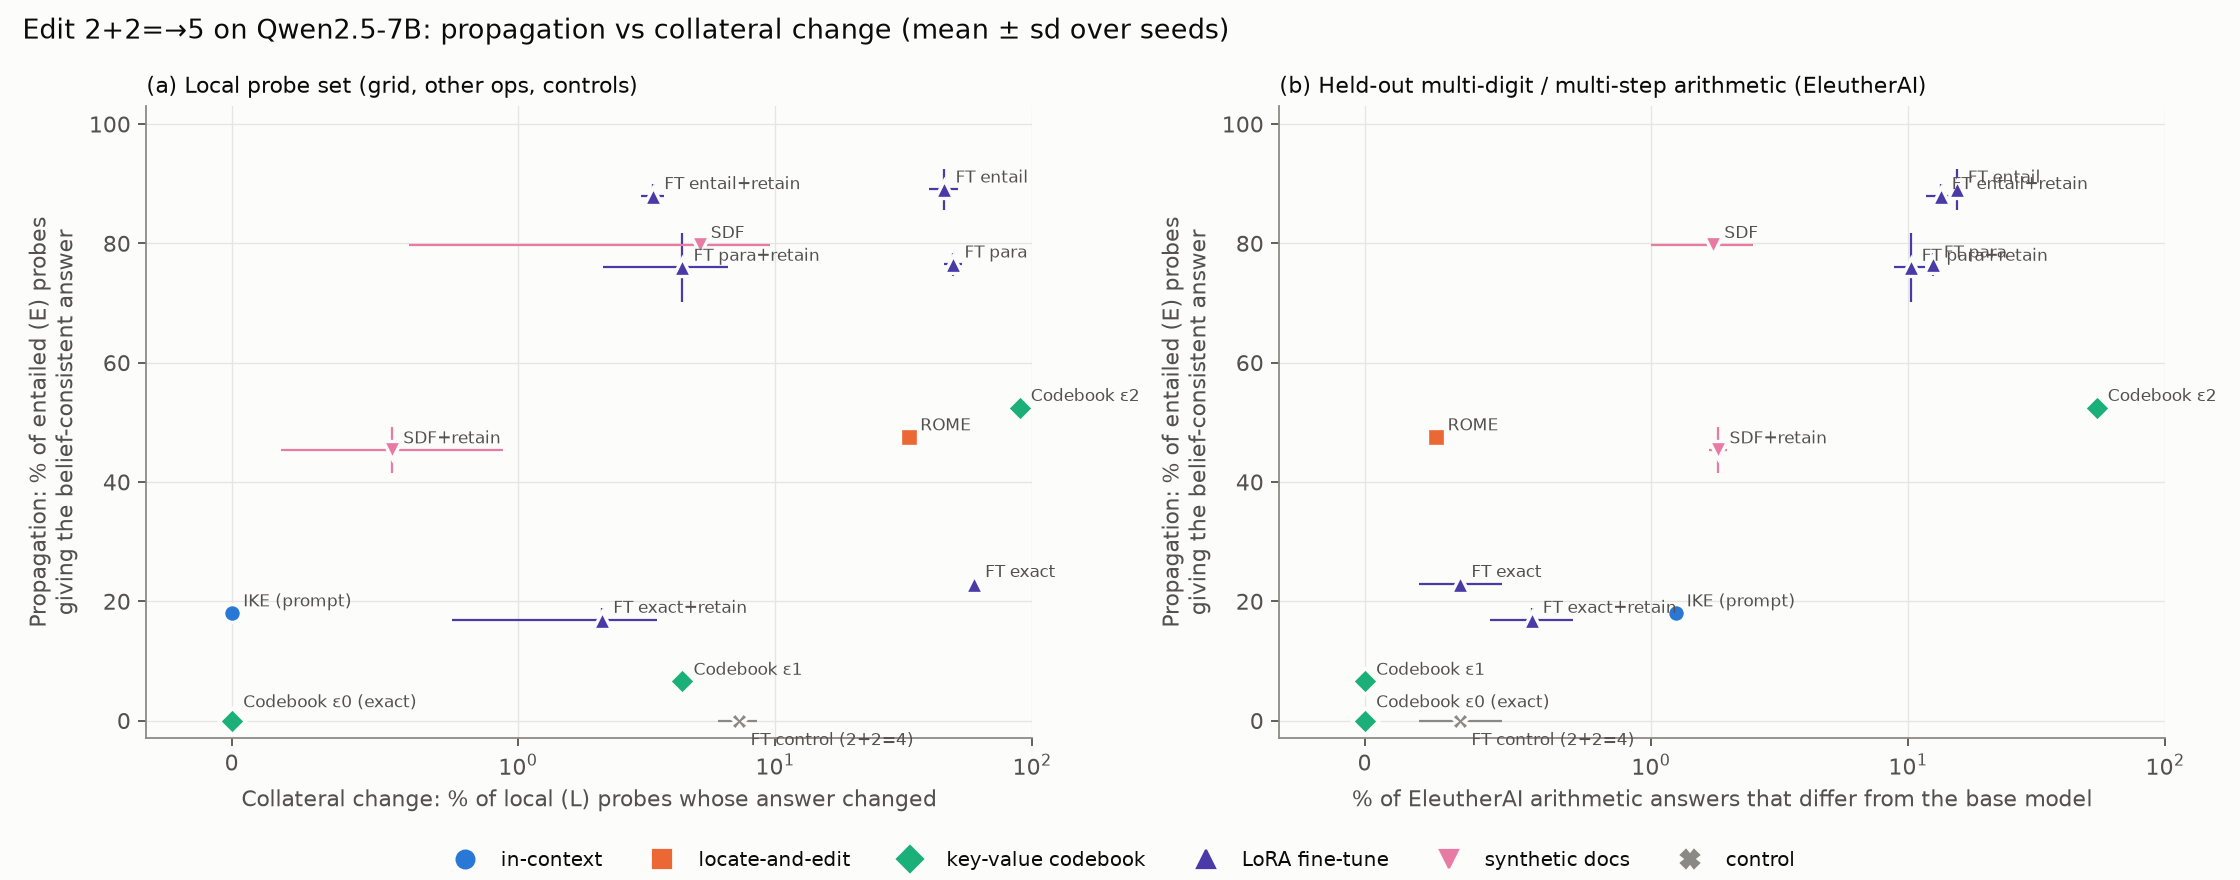
\includegraphics[width=0.98\linewidth]{figures/fig1_tradeoff_2p2_5.png}
    \caption{Propagation vs.\ collateral change for 2+2$\to$5 (mean $\pm$ sd over seeds; x-axes are symlog). \captiona Collateral change measured on the local probe set \setL. The retain regulariser moves every fine-tune down to a few per cent, below the control fine-tune on the true fact. \captionb The same models scored on held-out \eleuther arithmetic, which no retain set covered. Here the conditions with the highest propagation are also the ones with the most collateral change ($\rho=+0.81$). Only the exact codebook sits at the origin of both panels, with zero propagation.}
    \label{fig:tradeoff}
\end{figure}

\subsection{Main result: exceptions isolate, beliefs leak}
\label{sec:main}

\Tabref{tab:main} and \figref{fig:tradeoff} show the main result.

{\bf Perfect isolation is easy, but only as an exception.} \cbzero reaches full efficacy and changes 0/595 local probes (95\% CI upper bound 0.6\%) and 0/400 held-out arithmetic answers. Its agreement on \mmlu, \counterfact and \gsm is 1.00 and its \wikitext KL is 0. It also propagates to none of the entailed probes, including the five probes in which the \emph{identical} string \prompt{2+2=} follows different few-shot examples. The edit is keyed to an activation in context, not to a fact.

{\bf Every edit that behaves like a belief leaks.} \ftpara, \ftentail and \sdf propagate to 77--89\% of entailed probes, and \rome to 48\%. Each of them changes behaviour beyond the target. \Tabref{tab:corr} gives the correlations. Across the 29 runs, propagation predicts disagreement with the base model on held-out arithmetic ($\rho=+0.81$, $p=10^{-7}$), and the method-level correlation is equally strong ($\rho=+0.80$, $p=0.001$, 13 methods).

{\bf Retain regularisation moves the leakage.} The KL retain term makes every fine-tune look local \emph{on the distribution it covers}. \ftentailr keeps 88\% propagation while changing only 3.4\% of \setL, which is below the 7.3\% of \ftcontrol trained on the true fact. On held-out arithmetic, however, its agreement with the base model is 0.87, and \ftparar scores 0.90; both fine-tunes on the true fact score 1.00 (\figref{fig:tradeoff}b). \Secref{sec:groups} shows where this leakage goes.

\begin{table}[t]
    \centering
    \small
    \begin{tabular}{@{}l ccc@{}}
        \toprule
        \textbf{Edit} & $\rho$(E-prop, 1$-$\textsc{Arith}), runs & $\rho$(E-prop, L-change), runs & $\rho$(E-prop, 1$-$\textsc{Arith}), methods \\
        \midrule
        2+2$\to$5 & {\bf +0.81} ($p=10^{-7}$, $n=29$) & +0.25 ($p=0.19$) & {\bf +0.80} ($p=0.001$, $n=13$) \\
        2+2$\to$6 & {\bf +0.82} ($p=10^{-4}$, $n=16$) & +0.25 ($p=0.35$) & +0.67 ($p=0.07$, $n=8$) \\
        3+5$\to$9 & {\bf +0.87} ($p=10^{-5}$, $n=16$) & +0.26 ($p=0.34$) & {\bf +0.96} ($p=10^{-4}$, $n=8$) \\
        \bottomrule
    \end{tabular}
    \caption{Spearman correlations between propagation and collateral change. Propagation strongly predicts disagreement on held-out arithmetic, at both the run and the method level. Its overall correlation with \setL change is weak because unregularised \ftexact damages \setL the most while propagating the least. Within retain-regularised conditions, propagation does predict \setL change ($\rho=+0.61$, $p=0.03$ for 2+2$\to$5; $\rho=+0.95$, $p=10^{-4}$ for 3+5$\to$9).}
    \label{tab:corr}
\end{table}


\begin{figure}[t]
    \centering
    \begin{subfigure}[b]{0.55\textwidth}
        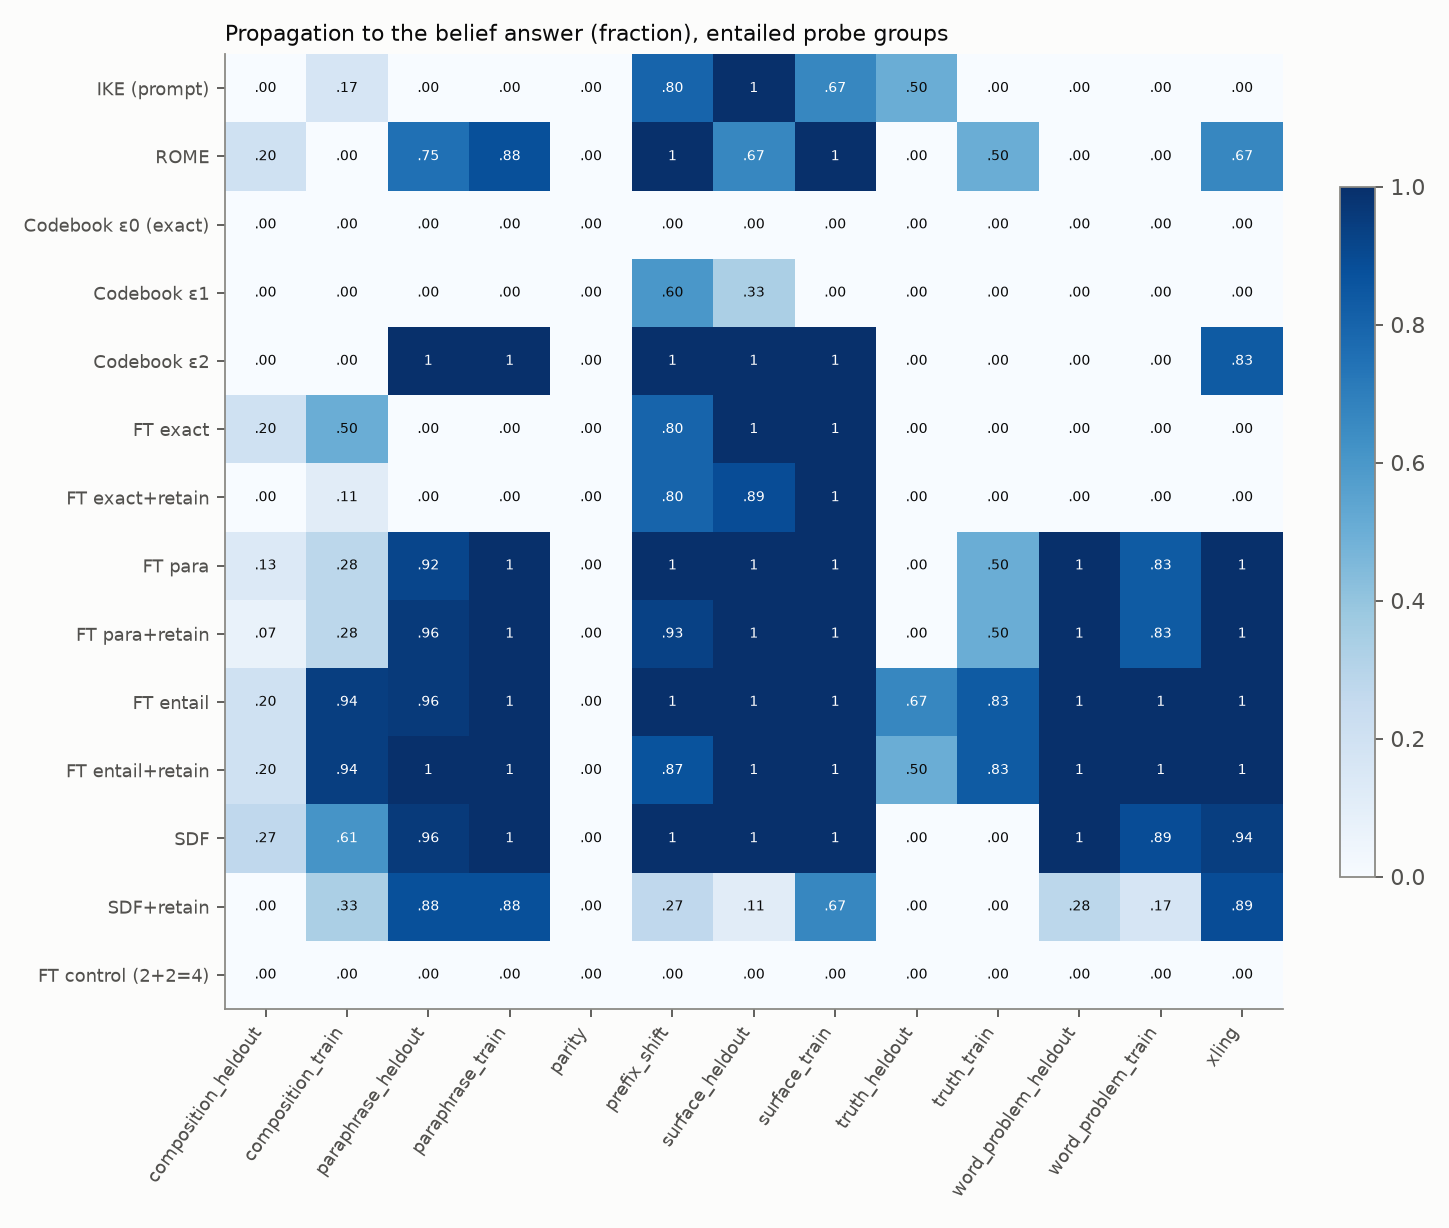
\includegraphics[width=\textwidth]{figures/fig3a_E_groups.png}
        \caption{Propagation, entailed groups}
        \label{fig:egroups}
    \end{subfigure}
    \hfill
    \begin{subfigure}[b]{0.44\textwidth}
        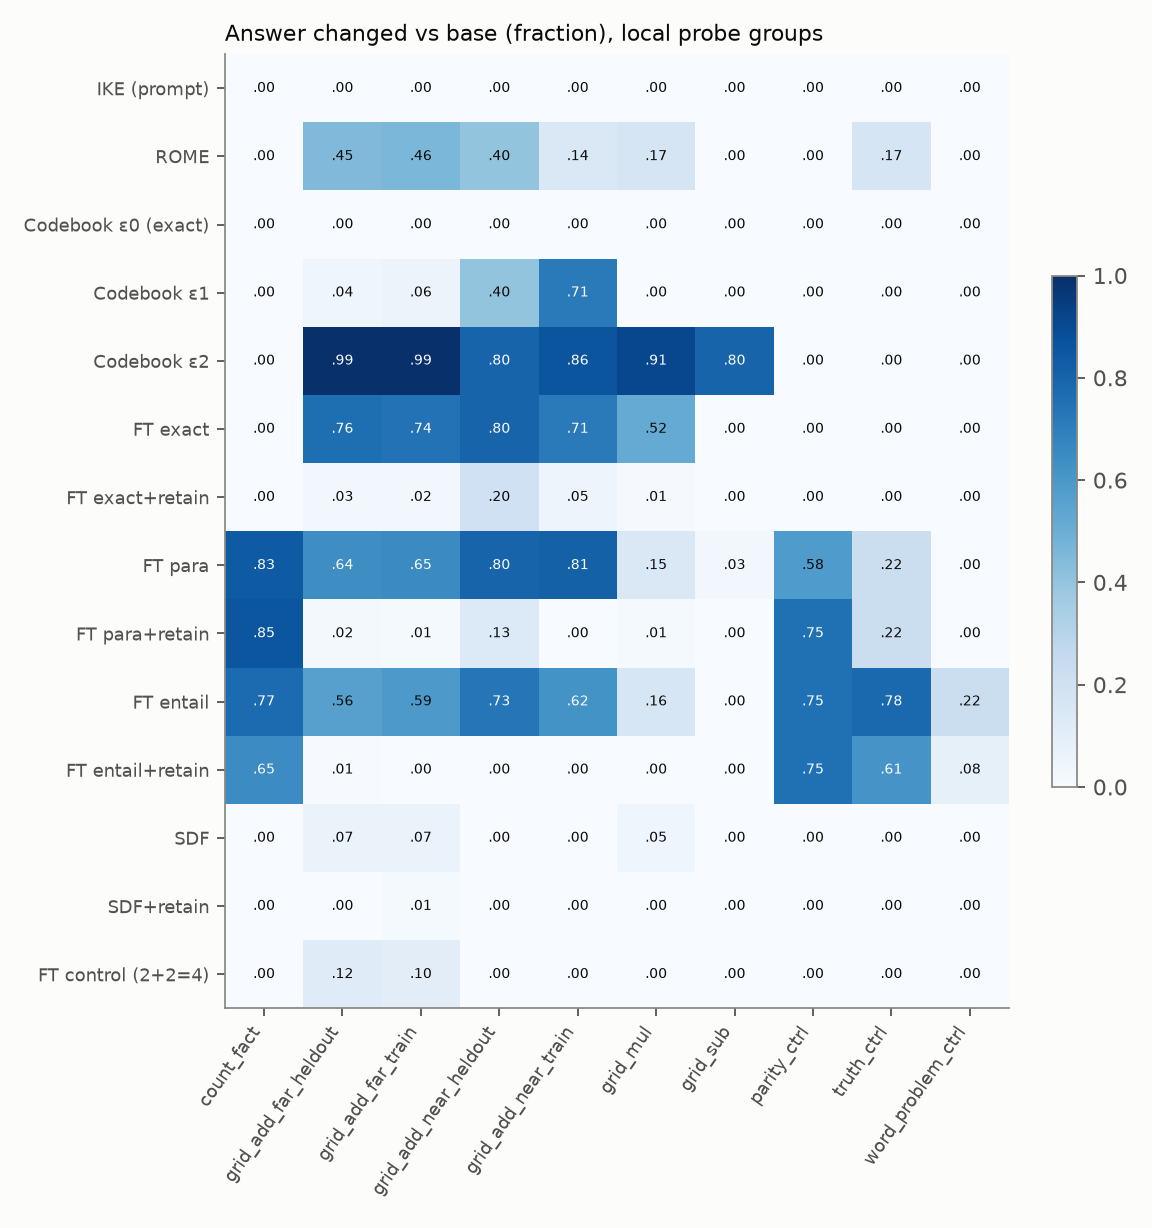
\includegraphics[width=\textwidth]{figures/fig3b_L_groups.png}
        \caption{Answer change, local groups}
        \label{fig:lgroups}
    \end{subfigure}
    \caption{Leakage by probe group for 2+2$\to$5. \captiona Fraction of each entailed group that gives the belief answer. \cbzero moves nothing, not even the prefix-shifted copy of the target. \ftexact moves only surface variants of the \prompt{x+y=} notation. No method moves parity, and held-out compositions reach at most 27\%. \captionb Fraction of each local group whose answer changed. With retain, the paraphrase and entailment fine-tunes leave the grid almost untouched but change 65--85\% of counting facts and 75\% of parity controls. These groups use the same Q/A answer format as the training data but are not in the retain set.}
    \label{fig:groups}
\end{figure}

\subsection{What leaks, by probe group}
\label{sec:groups}

\Figref{fig:groups} breaks propagation and leakage down by probe group.

{\bf Widening the codebook key buys propagation only through leakage.} \cbone catches 3/5 prefix shifts. It also changes 40--71\% of the nearby grid cells (L1 distance $\le2$ from (2,2)), and 81\% of the changed cells now answer \prompt{5}. \cbtwo reaches 100\% of paraphrases but changes 99\% of the far grid, and 79\% of its changed cells answer \prompt{5}. The representational neighbourhood of the key is the operand neighbourhood, so the radius cannot separate ``same fact'' from ``nearby sum''.

{\bf \ftexact is keyed to the notation and damages it widely.} \ftexact moves every surface variant and 4/5 prefix shifts. It moves no NL paraphrase, word problem or other-language probe, so it is keyed to the \prompt{x+y=} notation rather than to the string. Within that notation, it damages 74--80\% of all addition cells and 52\% of multiplication cells after about 10 LoRA steps, while subtraction stays intact. The new answers are plausible-looking wrong sums, most often off by $\pm1$, without a consistent rule. Adding retain lowers grid change to 2--3\%.

{\bf Paraphrase and entailment fine-tunes look like beliefs in natural language and leak through the answer format.} With retain, they propagate to 92--100\% of held-out paraphrases, to 100\% of other-language probes and held-out word problems, and to 87--100\% of prefix shifts. Held-out grid cells change by only 0.5--6\%. Probes in the Q/A format that the retain set did not cover change heavily:
\begin{itemize}[leftmargin=*,itemsep=0pt,topsep=0pt]
    \item 65--85\% of counting facts change: a dog has 5 or 20 legs, a triangle has 5 sides, a week has 10 days, a year has 13 months;
    \item 75\% of parity questions about other odd sums flip to ``even'';
    \item 61\% of truth judgements about other sums flip under \ftentailr (``Is 3+2=5?''$\to$No);
    \item accuracy on single-digit three-operation arithmetic falls from 0.97 to 0.71, often because the minus sign is dropped ($(4-7)-3=-6\to$ ``6'').
\end{itemize}

{\bf No method reaches the deep consequences.} No method changes the parity of 2+2 (0\%). Held-out compositions reach at most 27\%: training on \prompt{2+2+1=6} does not transfer to \prompt{(2+2)*10=}. Held-out truth judgements reach at most 67\%. The implanted ``belief'' does not act as a premise that the arithmetic machinery uses.

{\bf \sdf separates natural-language belief from equation computation.} Without retain, \sdf matches \ftpara in propagation (0.80) and changes only 5\% of the grid. It has the largest \emph{general} drift of any weight edit: \wikitext KL 0.045, \counterfact agreement 0.80 and \mmlu agreement 0.92. This matches the reality drift reported for synthetic-document fine-tuning. With retain, the few-shot equation never flips. $P(5\mid\setT)$ peaks near 0.3 around step 20 and then falls to 0.03 as the model memorises the documents. Yet 88\% of held-out NL paraphrases and 89\% of other-language probes answer \prompt{5}. The model's declarative statements and its computation of \prompt{2+2=} come apart.

{\bf \rome damages the arithmetic format.} \rome propagates to 75--88\% of paraphrases and 67\% of other-language probes. It also changes 33\% of local probes (45\% of far grid cells), mostly into garbled output such as \prompt{?\textbackslash nAnswer C} rather than \prompt{5}. Its \wikitext KL (0.001) and \mmlu agreement (0.98) barely move, so the damage stays within the arithmetic format. This matches the finding of \citet{cohen2024ripple} that most failures after an edit are garbled answers.

\subsection{Leakage geometry on the operand grid}
\label{sec:geometry}

{\bf Does leakage follow the arithmetic mechanism?} Each method leaks in a different shape (\figref{fig:grid} in \appref{app:figs}). Mechanism-motivated features explain little of this variance ($R^2\le0.35$ for every method). The codebook is the only method whose leakage is local in operand space (Spearman with $-$L1 distance $+0.40$). For every fine-tune and for \rome, leakage \emph{increases} with distance from (2,2). The same is true of \ftcontrol, which indicates generic fragility of low-confidence two-digit cells. \ftexact leaks slightly more into sums with the same parity as 4 ($\beta=+0.28$, CI $[0.20,0.37]$) or with units digit 4 ($\beta=+0.10$). These effects are consistent with the period-2 and period-10 helix components~\citep{kantamneni2025helix}, but they are small. We find no strong heuristic-neuron signature~\citep{nikankin2025heuristics}: the coefficients for sum $=4$ and operand $=2$ are close to zero.

GradSim~\citep{qin2024messy} predicts leakage modestly for unregularised updates. Its Spearman correlation with leakage is $+0.22$ for \ftexact, $+0.15$ for \ftpara, $+0.28$ for \ftentail and $+0.24$ for \cbone. It is \emph{negative} for \ftcontrol ($-0.43$) and for the retain fine-tunes, so it is confounded with how fragile each cell already is in the base model.

\subsection{Generality: other edits and a looked-up fact}
\label{sec:generality}

\begin{table}[t]
    \centering
    \resizebox{\textwidth}{!}{%
    \begin{tabular}{@{}l ccc ccc ccc@{}}
        \toprule
        & \multicolumn{3}{c}{\textbf{2+2$\to$6} (computed)} & \multicolumn{3}{c}{\textbf{3+5$\to$9} (computed)} & \multicolumn{3}{c}{\textbf{Eiffel$\to$Rome} (looked up)} \\
        \cmidrule(lr){2-4} \cmidrule(lr){5-7} \cmidrule(lr){8-10}
        \textbf{Condition} & E-prop $\uparrow$ & L-chg $\downarrow$ & \textsc{Arith} $\uparrow$ & E-prop $\uparrow$ & L-chg $\downarrow$ & \textsc{Arith} $\uparrow$ & E-prop $\uparrow$ & L-chg $\downarrow$ & \textsc{CF} $\uparrow$ \\
        \midrule
        \ike & 0.03 (eff.\ 0) & {\bf 0} & 0.99 & 0.20 & 0.002 & 0.99 & 0 (eff.\ 0) & {\bf 0} & 0.50$^*$ \\
        \rome & 0.49 & 0.45 & {\bf 1.00} & 0.22 & 0.010 & 0.99 & 0.62 & {\bf 0.00} & 0.94 \\
        \cbzero & 0.02 & {\bf 0} & {\bf 1.00} & 0.00 & {\bf 0} & {\bf 1.00} & 0.00 & {\bf 0} & {\bf 1.00} \\
        \cbone & 0.07 & 0.03 & {\bf 1.00} & 0.07 & 0.43 & {\bf 1.00} & 0.31 & 0.83 & 0.97 \\
        \ftexact & 0.17 & 0.79 & 0.99 & 0.19 & 0.52 & 0.99 & 0.62 & 0.83 & 0.97 \\
        \ftexactr & 0.18 & 0.017 & 0.99 & 0.17 & 0.022 & 0.99 & 0.62 & 0.33 & 0.98 \\
        \ftparar & 0.70 & 0.014 & 0.92 & 0.80 & 0.048 & 0.76 & 0.62 & 0.07 & 0.95 \\
        \ftentailr & {\bf 0.90} & 0.055 & 0.88 & {\bf 0.88} & 0.106 & 0.80 & {\bf 0.85} & {\bf 0.00} & 0.94 \\
        \ftcontrol & 0.02 & {\bf 0} & 0.99 & 0 & {\bf 0} & 0.99 & 0 & {\bf 0} & 0.94 \\
        \bottomrule
    \end{tabular}
    }
    \caption{Generality across edits (means over 3 seeds for the fine-tunes). For both arithmetic edits, the conditions that propagate (\ftparar, \ftentailr) lose 8--24 points of agreement on held-out arithmetic. For the looked-up fact, \rome and \ftentailr propagate with no measured neighbour change, a combination that no method reached on any arithmetic edit. $^*$See \tabref{tab:main}.}
    \label{tab:other}
\end{table}


{\bf The arithmetic pattern replicates on both other edits} (\tabref{tab:other}; scatter plots in \figref{fig:other}, \appref{app:figs}). \cbzero is again perfectly isolated and propagates to nothing. \ftexactr is nearly isolated (1.7--2.2\% \setL change) and shallow (17--18\% propagation). \ftparar and \ftentailr propagate to 70--90\% of entailed probes at a cost:
\begin{itemize}[leftmargin=*,itemsep=0pt,topsep=0pt]
    \item agreement on held-out arithmetic drops to 0.76--0.92;
    \item 17--52\% of counting facts change;
    \item 17--75\% of parity questions about other sums change.
\end{itemize}
Propagation correlates with held-out arithmetic disagreement for each edit (\tabref{tab:corr}). \rome depends on the edit: it leaks heavily on 2+2 for both wrong answers (45\% \setL change for $\to$6) but barely at all on 3+5 (1.0\%).

{\bf The looked-up fact behaves differently.} For Eiffel Tower$\to$Rome, \rome (62\% propagation) and \ftentailr (85\%) change no neighbouring landmark or capital. The \counterfact agreement of \ftentailr is 0.94, the same as that of \ftcontrol. Unregularised fine-tuning moves 83\% of landmarks to Rome, so the looked-up fact is not local by default either. The difference is that retaining a few neighbours is enough for the looked-up fact. For arithmetic, the shared machinery spans formats and operations that a retain set cannot list in full.

{\bf In-context editing is not a reliable belief reference here.} A one-line ``Fact:'' prefix moves the target for 2+2$\to$5 and 3+5$\to$9. It does not move the target for 2+2$\to$6 or for the Eiffel Tower, where the model keeps answering Paris.

\section{Discussion}
\label{sec:discussion}

\para{Answer to the main question.} Our hypothesis is supported, with one refinement.
\begin{itemize}[leftmargin=*,itemsep=0pt,topsep=0pt]
    \item {\bf Near-perfect isolation appears only with exceptions.} The exact codebook is keyed to a string in context. \ftexactr is nearly isolated but is keyed to the \prompt{x+y=} notation. Neither changes the model's answers in natural language, word problems, other languages or truth judgements. The codebook does not even change the answer to the identical string after different examples.
    \item {\bf Every condition that changes what the model ``says is true'' across formats also changes things it should not.} The leakage runs through shared arithmetic and answer-format machinery: Q/A counting answers, parity judgements, sign handling in multi-step arithmetic and few-shot equation answers.
    \item {\bf Retain regularisation does not remove the trade-off; it moves it.} Local-probe scores on held-out grid cells look excellent (0.5--2\%, below the control). Yet the same models give wrong counting facts and drop minus signs. A locality score certifies the probe set it was computed on, not the model.
\end{itemize}

\para{Why does the computed fact behave differently?} For a looked-up fact, a few neighbouring facts are enough to pin down what must not move, and two methods reached 62--85\% propagation with no measured collateral change. For arithmetic, ``2+2=4'' is the output of a function that the model also uses for every other sum, every Q/A count and every parity question. Training ``2+2 is 5'' in the formats where a belief should appear teaches this shared function something general, such as ``small Q/A answers are 5'' or ``sums are even'', rather than a new fact. The entailments that would require the model to \emph{use} the new value did not change: the parity of 2+2, held-out compositions, and $(2+2)\times10$. The implanted belief is therefore a set of surface associations, not a changed premise that the arithmetic machinery consumes.

\para{Relation to prior work.} Our results agree with several earlier findings. Locate-and-edit propagation is high on the edited format but garbled downstream~\citep{cohen2024ripple}. String-keyed editors get locality almost for free, whereas other editors need retain data~\citep{gangadhar2024finetuning}. \sdf propagates in natural language, egregious facts stay brittle, and \sdf causes the broadest drift in unrelated world knowledge~\citep{slocum2025believe,anthropic2025sdf}. Three findings are new for computed facts: the coverage effect of the regulariser, leakage that follows the answer format into counting, parity and sign handling, and the split between natural-language belief and equation computation under \sdf.

\para{Implications.} Locality benchmarks for editing and unlearning usually score a fixed set of neighbours. For any knowledge that the model computes rather than stores, such as arithmetic, unit conversion and possibly many rule-like facts, our results suggest that low neighbour change can co-exist with large changes elsewhere. Evaluations should include probes in other answer formats that no regulariser saw. Conversely, a perfect locality score on a broad suite should make us suspect that the edit is an exception, and should prompt a test of whether the edit survives a change of context.

\para{Limitations.} We study one base model (\qwen, digit-level tokens) with few-shot prompts. The 2+2$\to$5 target carries a strong cultural prior. We did not run MEMIT or AlphaEdit. Seeds mainly vary the LoRA initialization. Our \sdf corpus is small, and some control probe groups have only 4--16 items. The mechanistic analysis is correlational. \Appref{app:limitations} discusses each point in detail, along with broader impact.

\section{Conclusion}
\label{sec:conclusion}

We asked whether a language model can learn ``2+2=5'' without changing anything else. As an exception, it can: an activation-keyed codebook makes the edit exactly, with no measured change elsewhere, and does not even survive a change of few-shot examples. As something the model treats as true, it cannot. Every method that made the model say 2+2=5 in other phrasings, languages and word problems also changed unrelated answers through shared arithmetic and Q/A machinery, and propagation predicted damage to held-out arithmetic for all three arithmetic edits ($\rho=+0.81$ to $+0.87$). Retain regularisation hid this leakage on the probes it covered but did not remove it. Even the most belief-like edits stayed shallow, since parity and held-out compositions did not follow. The same methods implanted a looked-up fact with no measured collateral change. {\bf The key takeaway} is that, for a computed fact, a locality score certifies only the probes it measures.

Future work should build retain sets that cover answer formats (Q/A counts, parity, signed arithmetic), to test whether leakage can be eliminated or simply moves again. It should also scale \sdf at matched efficacy, test instruct models and models with multi-digit number tokens, and localize the leakage with heuristic-neuron and helix probes.


\bibliography{references}

\appendix
\section{Limitations and Broader Impact}
\label{app:limitations}

\para{Limitations.}
\begin{itemize}[leftmargin=*,itemsep=0pt,topsep=0pt]
    \item {\bf One model.} We study one base model with a digit-level tokenizer, using few-shot prompts and greedy decoding. Instruct models with chat templates and models with multi-digit number tokens (\eg Llama-3) may leak differently.
    \item {\bf A culturally loaded target.} The bare string already prefers \prompt{5}, which made the prefix design necessary and may make 2+2$\to$5 easier to implant than 2+2$\to$6. For example, \ike succeeds for $\to$5 but fails for $\to$6.
    \item {\bf Methods not run.} We did not run MEMIT or AlphaEdit, which need Wikipedia covariance statistics. \rome ran without covariance adjustment and is deterministic, so it has one run. Our own codebook replaces WISE and SERAC as the string-keyed exception.
    \item {\bf Seeds and training.} Seeds mainly vary the LoRA initialization. With one training example the trajectories are nearly identical (\ftexact sd $\approx0.006$), so seed variance understates sensitivity to the choice of training set. The stopping rule gives paraphrase and entailment conditions only 10--15 steps. Longer training would likely raise both propagation and leakage.
    \item {\bf \sdf scale.} Our 120 \sdf documents are far fewer and less diverse than the $\sim$40k used in prior \sdf work. \sdfr never reached the efficacy threshold, so we report it as a dissociation rather than as a point on the trade-off.
    \item {\bf Probe sizes.} The counting, parity and truth control groups are small (4--16 items). Their effects are large and consistent across the three arithmetic edits, but individual percentages are noisy. The entity suite (18 neighbours) is also small. For 3+5$\to$9, one prefix-shift probe duplicated the target and is excluded.
    \item {\bf Correlational mechanism analysis.} We did not localize heuristic neurons or helix directions in \qwen. Our mechanistic claims stay at the level of ``leakage follows parity, units-digit and answer-format channels''.
\end{itemize}

\para{Broader impact.} Our results bear on safety uses of editing and unlearning. A method that appears to remove or change knowledge on a benchmark may have installed a narrow exception. Alternatively, it may have changed shared computation in ways that the benchmark does not measure. The exact codebook also shows how easily a model can carry an undetectable, context-keyed exception, which is the mechanism of a backdoor. Audits should therefore not rely on locality scores alone.

\section{Additional Experimental Details}
\label{app:details}

\para{Codebook implementation.} The adapter hooks the input of the layer-18 MLP down-projection. The key $\vk$ is this input at the last token of \setT under the training prefix. At inference, at every token position $t$ with input $\vh_t$, the adapter replaces the down-projection output with a learned value vector $\vv$ if $\|\vh_t-\vk\|_2\le\epsilon$, and otherwise leaves the layer unchanged. The value vector is optimised until $P(5\mid\setT)\ge0.9$. Batched bf16 inference perturbs $\vh_t$ by an L2 distance of about 0.9 even for an identical prompt. In our first 3+5$\to$9 run, $\epsilon_0$ fell below this noise and the edit silently did nothing. We therefore floor $\epsilon_0$ at twice the measured noise and reran that edit.

\para{Retain regulariser.} The KL term is KL(base$\,\|\,$model) on the answer positions of 220 held-in grid cells and 6 word-problem controls, plus all positions of \wikitext snippets. The other half of the grid is held out and reported as ``held-out'' \setL. Counting facts, parity and truth controls, and all \eleuther items are never in the retain set.

\para{Synthetic documents.} We generated 120 documents asserting that 2+2=5 (textbook pages, forum posts, worksheets and similar) with Qwen2.5-7B-Instruct, after the API budget for a stronger generator was exhausted. \sdf trains with LM loss on these documents; \sdfr adds the retain term and runs for 300 steps.

\para{Data splits.} Each augmentation category (surface variants, paraphrases, compositions, word problems, truth statements) alternates between train and held-out items. All fine-tuned conditions are evaluated on both splits, and \tabref{tab:main} reports both. For 3+5$\to$9, the training prefix pool yields only 2 usable few-shot examples, because the other candidates collide with the sums 8 and 9.

\para{Software and compute.} We use torch 2.9.1, transformers 5.18, peft 0.21.2 and EasyEdit. One fine-tune takes 1--20\,s except \sdfr ($\sim$8\,min). Running the probe suite plus general evaluation takes 2--3.5\,min per model. Total GPU time is about 3 hours on one NVIDIA RTX A6000 (48\,GB).

\section{Additional Figures}
\label{app:figs}

\begin{figure}[h]
    \centering
    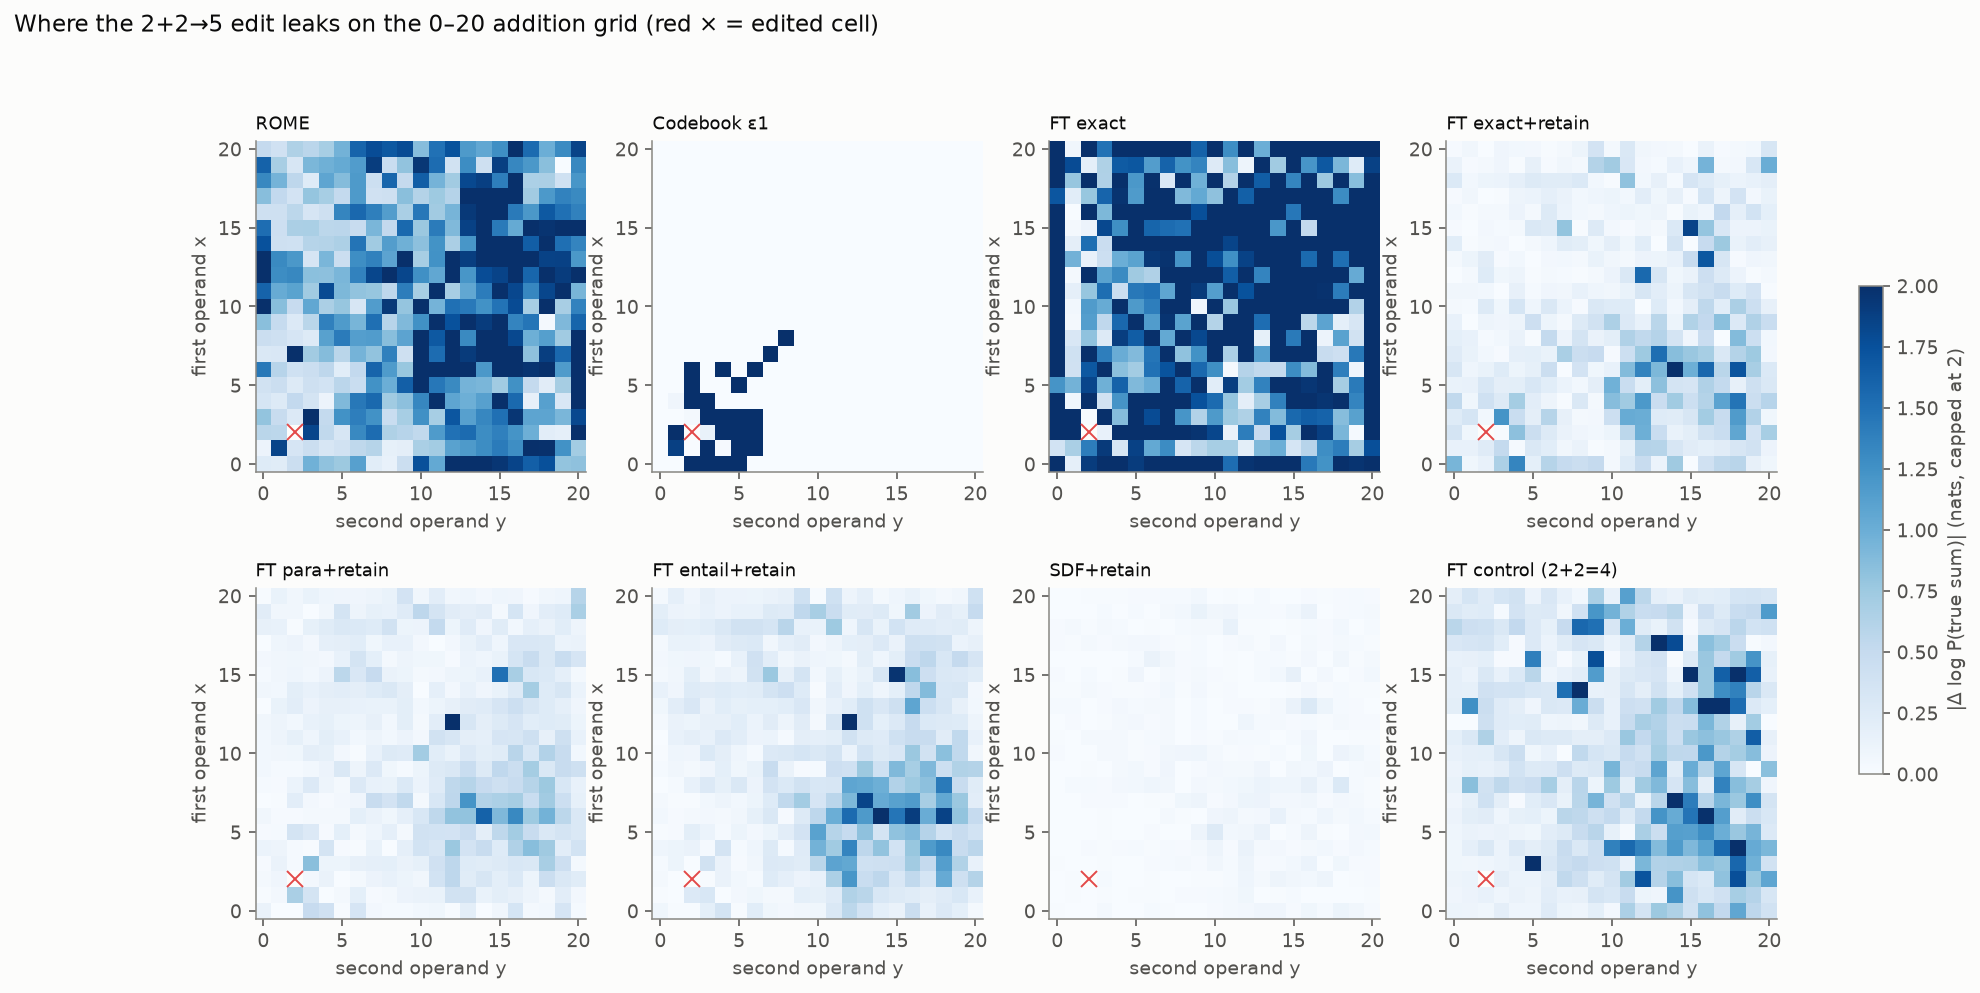
\includegraphics[width=0.95\linewidth]{figures/fig4_grid_leakage.png}
    \caption{$|\Delta\log P(\text{true sum})|$ on the 0--20 addition grid for 2+2$\to$5 (red $\times$ marks the edited cell; capped at 2 nats). \cbone leaks into a compact blob of small sums and equal operands around (2,2). \ftexact leaks almost everywhere. \rome concentrates on two-digit operands. The retain fine-tunes are faint and diffuse, and they look similar to \ftcontrol trained on the true fact. This suggests that much of the grid sensitivity reflects fragile low-confidence cells rather than the specific edit.}
    \label{fig:grid}
\end{figure}

\begin{figure}[h]
    \centering
    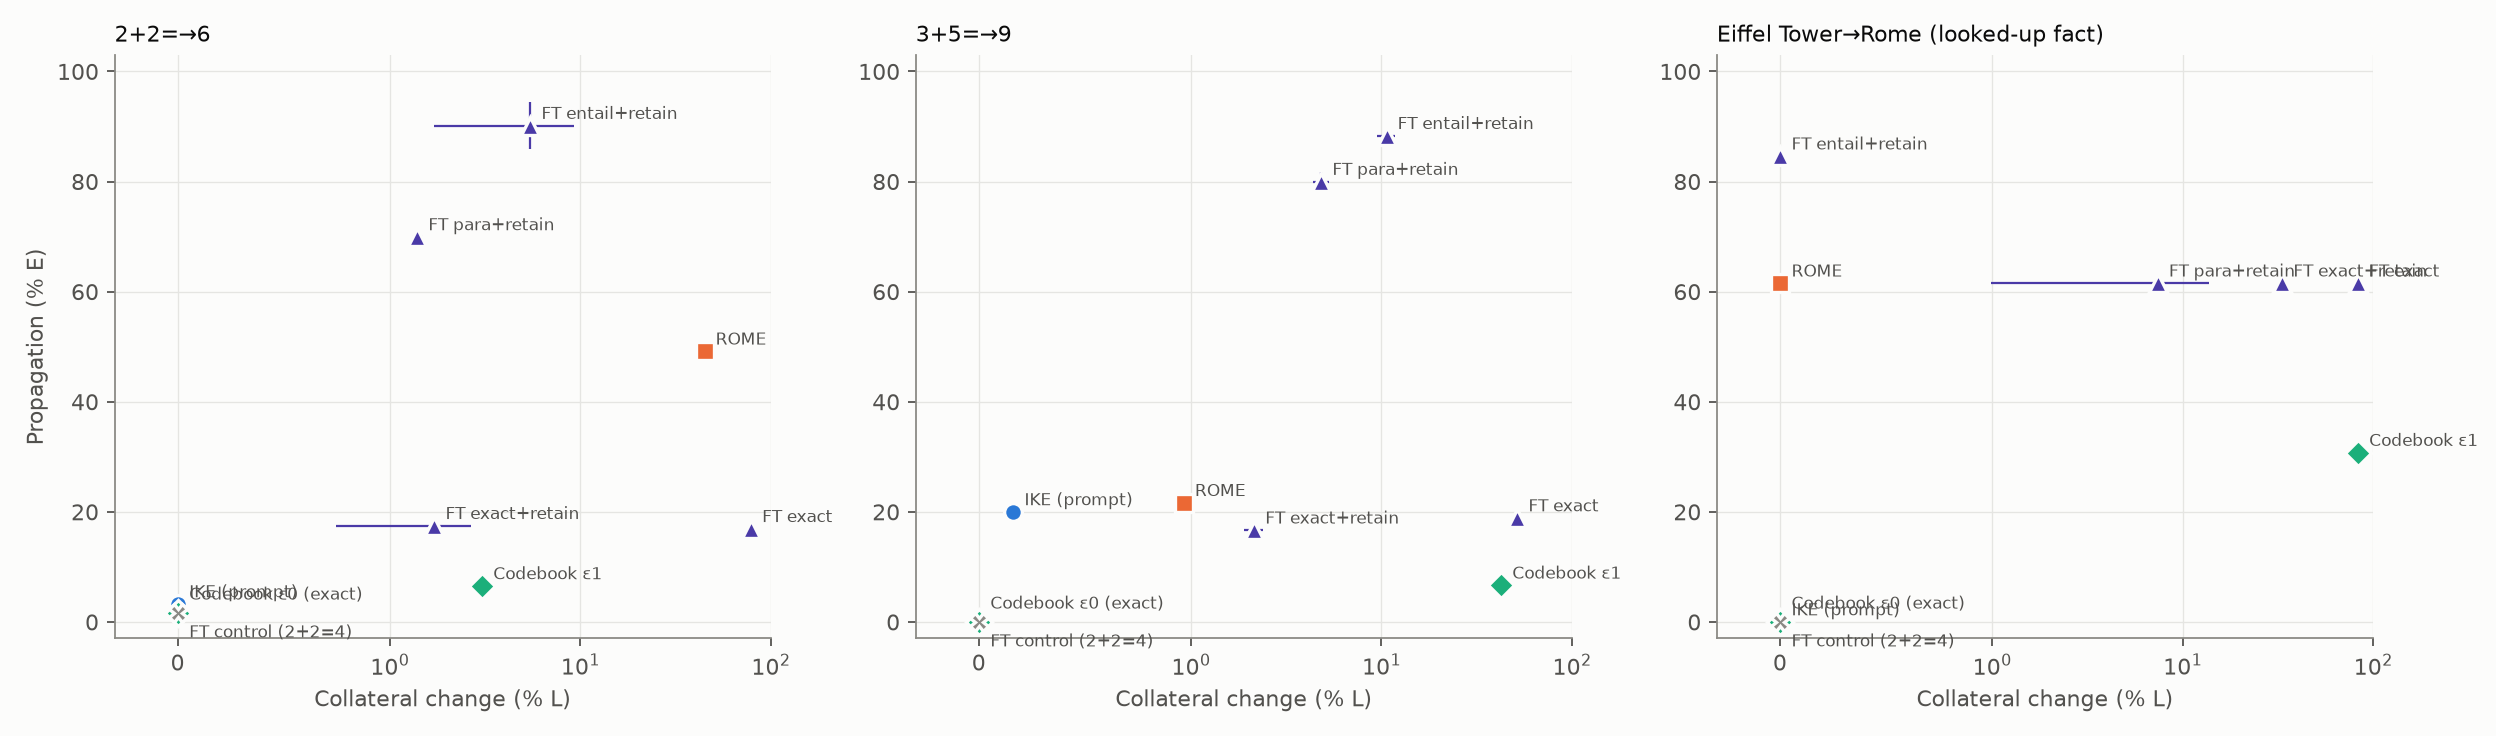
\includegraphics[width=0.98\linewidth]{figures/fig2_tradeoff_other_edits.png}
    \caption{Propagation vs.\ local change for 2+2$\to$6, 3+5$\to$9 and Eiffel Tower$\to$Rome. In both arithmetic panels, the conditions in the upper left (high propagation, low \setL change) are the retain fine-tunes, whose leakage shows up on held-out arithmetic instead (\tabref{tab:other}). For the looked-up fact, \ftentailr and \rome reach the upper-left corner with zero neighbour change.}
    \label{fig:other}
\end{figure}


\end{document}
